
\documentclass[12pt]{article}
\usepackage[utf8]{inputenc}	
\usepackage[T1]{fontenc}
\usepackage{lmodern}
\usepackage[francais]{babel}
\usepackage[separate-uncertainty = true]{siunitx}
%\usepackage{lscape}
%\sisetup{locale = FR}		
\usepackage{graphicx}
\usepackage{caption}
\usepackage{subcaption}
\usepackage{amsmath}
\usepackage{amsfonts}
\usepackage{xfrac}
\usepackage[section]{placeins}
\usepackage[top=2.5cm, bottom=2.5cm, left=2.5cm, right=2.5cm]{geometry}
\usepackage{float}
\usepackage{parskip}
\usepackage{color}
\usepackage{multicol}
\setlength{\parindent}{1cm}
\addto\captionsfrench{\def\tablename{Tableau}}
\addto\captionsfrench{\def\figurename{Figure}}
\usepackage{microtype}
%\usepackage[space]{grffile}
\usepackage{enumitem}
%\usepackage{multirow}
\usepackage{booktabs}
%\sisetup{round-precision=3,round-mode=figures,scientific-notation=true}
\usepackage{graphicx}
\usepackage{graphics}
\usepackage{subcaption}
\usepackage{mwe}
\usepackage{url}
\usepackage{titletoc}
\usepackage{adjustbox}
\titlecontents{subsubsection}
  [0pc]
  {\addvspace{1.5pc}\bfseries}
  {\thecontentslabel\hspace{0.8em}}
  {}
  {}
  []



\title{Data Analysis: Chunk size determination for HPX parallel for-loops }

\begin{document}


\pagenumbering{roman}
\pagenumbering{arabic}
%%%%%%%%%%%%%%%%%%%%%%%%%%%%%%%%%%%%%%%
%\tableofcontents

\newpage
\section*{Project Overview}
 In today's day and age, we are constantly trying to optimize our algorithms to improve performance and minimize execution time. One of the ways we can achieve those goals is by using loop-level parallelism. If an algorithm is made of independent iterations, such a technique can be used. Using HPX's $for\_each()$ algorithm, the different iterations are assigned to threads and then to different CPU's. One of the key parameters of parallelization is chunk size which, in that case, represent how much work is assigned to a single thread.
The goal of this project is to be able to predict the optimal chunk size for a given task. \\

One method that has proven to be successful to predict such parameters is machine learning. In machine learning, you train a model based on data to get predictions on new situations. The first section will focus all the notation used during the document.
\section{Mathematical Notation}
The ultimate goal of this research is to minimize the execution time of a parallel loop. Here is an example of a hpx for loop. 

\begin{figure*}[h]
	\centering
	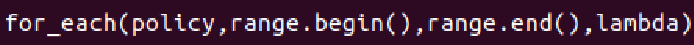
\includegraphics[scale=0.8]{images/for_each_call.pdf}
\end{figure*}

In such loops, a lambda function is applied over a range. The lambda function could be any algorithm such as, for instance, matrix multiplication. Each instance of a loop being run will be referred to as an experiment. Each experiment has an unique set of features which will be called $X_i$ for the $i$th experiment. The following six features are used:

\begin{itemize}
	\item[1] <Total Number of operations per iteration>
	\item[2] <Number of float operations per iteration>
	\item[3] <Number of comparison operations per iteration>
	\item[4] <Deepest loop level>
	\item[5] <Input size (range)>
	\item[6] <Number of threads>
\end{itemize}

The first four features will be considered static since they only depend on the lambda function internal structure. They are collected at compile time by a ClangTool called loop convert.

The last two are dynamic since they do not depend on the algorithm and are extracted at run-time.

If we assume that the variance in time measurement is small, we can say that time is a function of features and chunk size. If the set of all possible features is denoted by $\{X_i\}$ and the set of all possible chunk sizes by $CS$ then we have:

$$t:\{X_i\} \otimes CS \rightarrow \mathbb{R}$$

$\otimes$ is a tensorial product which means that time is a function of both features and chunk size.
Our ultimate goal is to find the chunk size that minimizes the execution times for a given set of features. This means that we want to find the function:

\begin{equation}
	f(X_i)=\underset{cs \in CS}{\arg\min} \, \, t(X_i,cs)=cs_i
\end{equation}


The  value $cs_i$ is known as the optimal chunk size as it minimizes the execution time for experiment $i$. $f$ is the function that outputs the optimal chunk size of a given loop. Optimal chunk sizes will be referred to as target values which is the vocabulary used in machine learning for values that we want to predict.

The objective is to use machine-learning algorithms to approximate the function f (1).

\section{Data Description}
The data that must be generated is comprised of features and target values. $(X_i,cs_i) \, \, \, \forall i$. To generate different features, one needs to use multiple lambda functions and apply then on different ranges.

In practice, how does one find the target value for an experiment? We can find the target value $cs_i$ by applying equation [1], but finding the minima is impossible since the set $CS$ of all possible chunk sizes is very large. The idea that was used in [0] was to restrict $CS$ to a small set
$CS=\{0.001;0.01;0.1;0.5\}$. Each value in the set is referred to as a candidate. Having a small set means that you don't have the absolute best chunk size but an approximation of it. Even though its an approximation it will still be referred as $cs_i$
Note that here the chunk size is a percentage which represent what fraction of the total number of iterations is given to a thread. In that instance $\frac{1}{cs_i}$ represents the number of chunks in which you divide your job. To resume, generating target values consist of choosing a finite set $CS$ of candidates and apply equation (1) which means evaluating the execution time for all candidates and taking the chunk-size with minimal time as target value for the experiment.


\subsection{Data Generation}
Data generation consist of running experiments and extract the values $(X_i,cs_i) \, \, \, \forall i$. the features of loops are extracted at compile and run-time and the execution time are measured for different chunk sizes candidates. 

Here is an example of a data-set comprised of three different experiments and $CS=\{0.001;0.005;0.01;0.05;0.1;0.2;0.5\}$

\begin{figure*}[h]
	\centering
	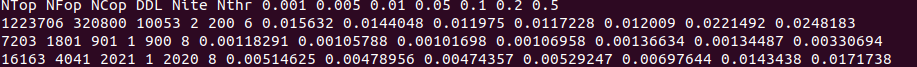
\includegraphics[scale=0.45]{images/screenshot_data.png}
\end{figure*}


Here is a pseudo code of how the data is generated.

\begin{figure*}[h]
	\centering
	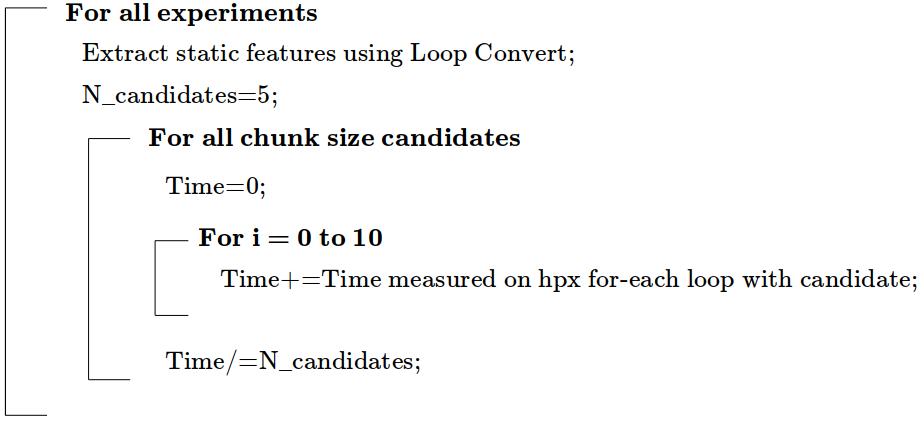
\includegraphics[scale=0.49]{images/pseudo-code.png}
\end{figure*}
\section{Data Analysis}

\subsection{Matrix Multiplication}
In this section, we will focus on the Matrix Multiplication algorithm. All experiments shown will have been run with a matrix multiplication lambda function in a HPX $for\_each()$ The goal is to start analyzing a smaller data set before slowly expanding it by adding new lambda functions. In the case of a matrix multiplication algorithm the feature <Input-size> can be renamed <Matrix Size>.

\subsubsection{Variance of execution times for a given chunk-size}
For a given experiment, you expect to get similar execution times for a given chunk size value every time you run it. There will always be some noise in the data since there are many processes that the user cannot directly control. To correct that, every for-loop is run $N_\text{rep}$ times and the execution time is given by the mean of these repetitions. Each repetition can be represented by an index $j=0,1,2,3,4, \dots$ So for an experiment $i$ the execution time outputted is 
$$\bar{t}_i=\frac{1}{N_\text{rep}}\sum_{j=1}^{N_\text{rep}}t_j$$
Note that the first repetition of the for-loop is ignored so this repetition could be given an index $j=0$. This is done to ignore the time where the cache memory is being filled.
One would expect the variance of the mean
to decrease as the number of repetitions get bigger. If this could be confirmed experimentally, this would mean that by taking more and more repetitions, one can get more precise in execution time measurement and therefore the data generation process described earlier can be reliable. Studying the variance is a great tool to measure the variations of execution time between repetitions but it does not inform on how much the values vary relative to their size. To solve this issue, the relative variance is used:
$$\operatorname{RelVAR}(\bar{t}_j)=\frac{\operatorname{VAR}(\bar{t}_j)}{\bar{t}_j^2}\times 100 \%$$

To test this assertion, the relative variance of the mean of execution times has been measured for values of $N_{rep}=10,25,50,75,100$. These measurements have been done on matrix multiplications algorithms with different number of threads and different matrix sizes
\begin{figure*}
	\centering
	\begin{subfigure}[b]{0.475\textwidth}
		\centering
		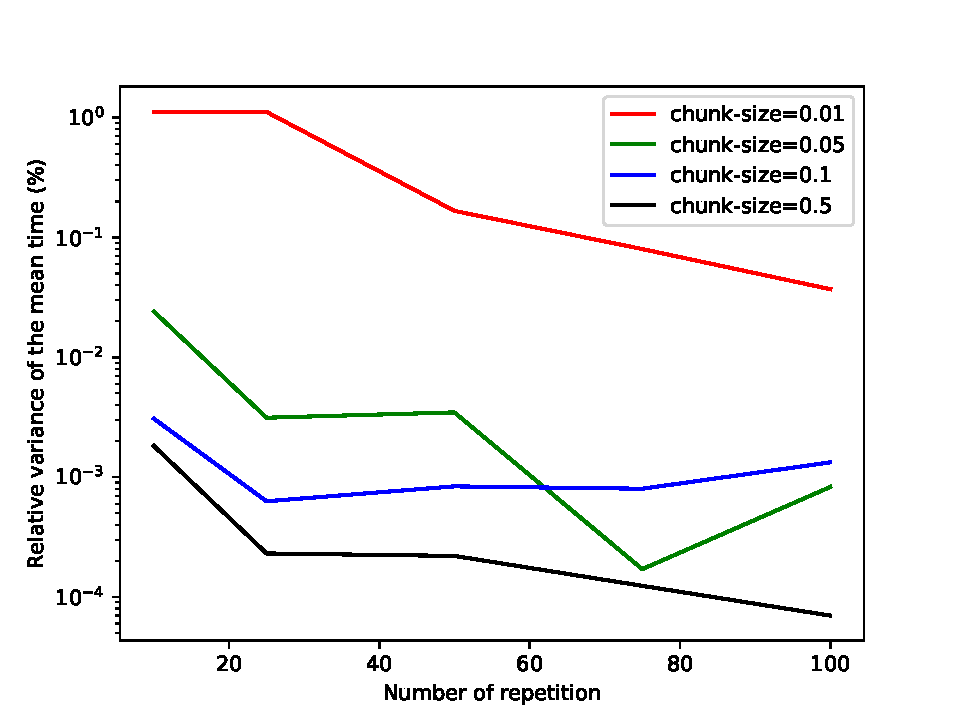
\includegraphics[width=\textwidth]{images/relvar_100_2.pdf}
		\caption[Network2]%
		{{\small 100$\times$100 on 2 threads}}    
	\end{subfigure}
	\hfill
	\begin{subfigure}[b]{0.475\textwidth}  
		\centering 
		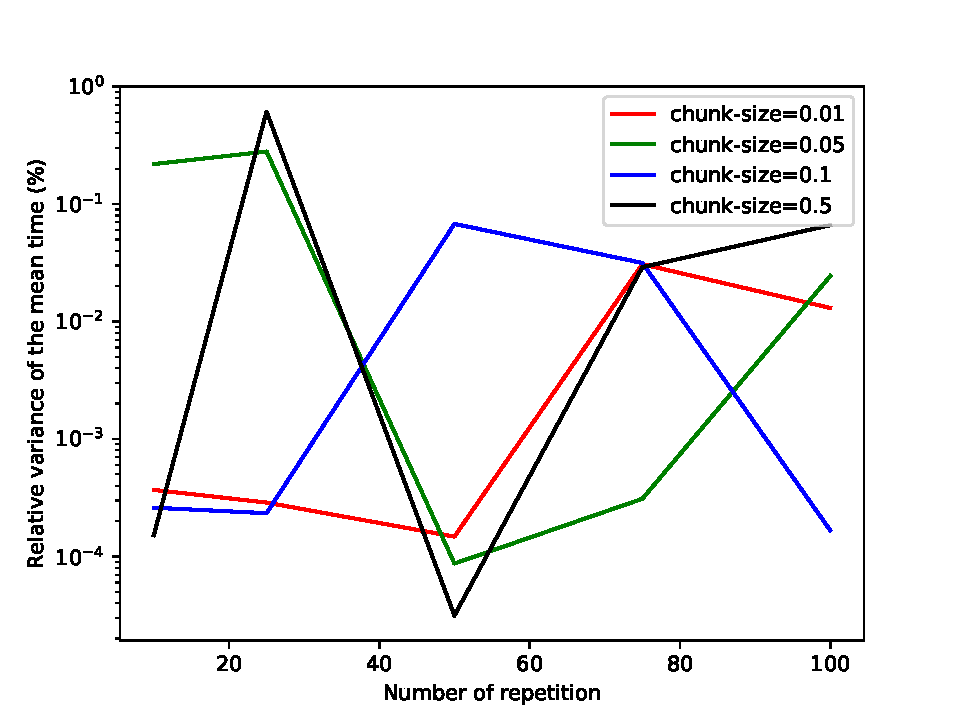
\includegraphics[width=\textwidth]{images/relvar_500_2.pdf}
		\caption[]%
		{{\small 500$\times$500 on 2 threads}}    
	\end{subfigure}
	\vskip\baselineskip
	\begin{subfigure}[b]{0.475\textwidth}   
		\centering 
		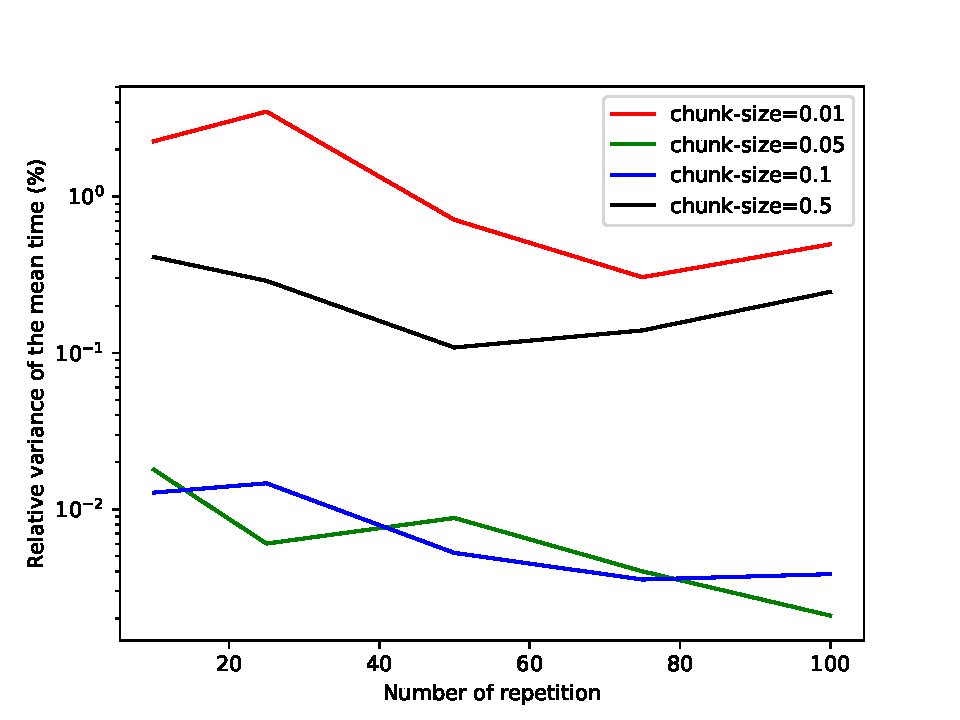
\includegraphics[width=\textwidth]{images/relvar_100_4.pdf}
		\caption[]%
		{{\small 100$\times$100 on 4 threads}}    
	\end{subfigure}
	\quad
	\begin{subfigure}[b]{0.475\textwidth}   
		\centering 
		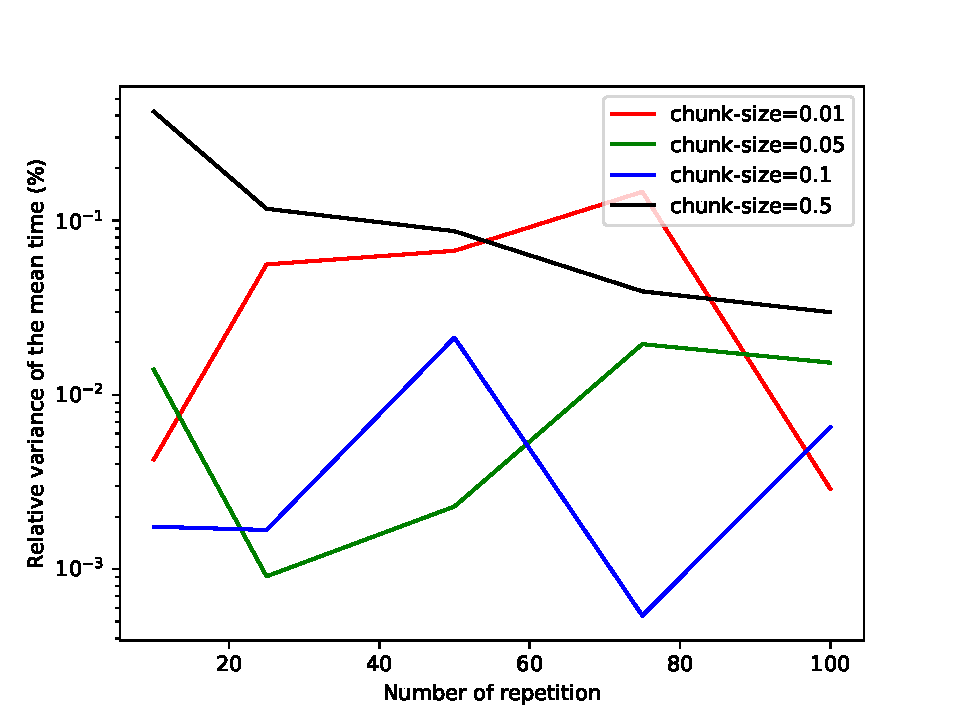
\includegraphics[width=\textwidth]{images/relvar_500_4.pdf}
		\caption[]%
		{{\small 500$\times$500 on 4 threads}}    
	\end{subfigure}
	\vskip\baselineskip
	\begin{subfigure}[b]{0.475\textwidth}   
		\centering 
		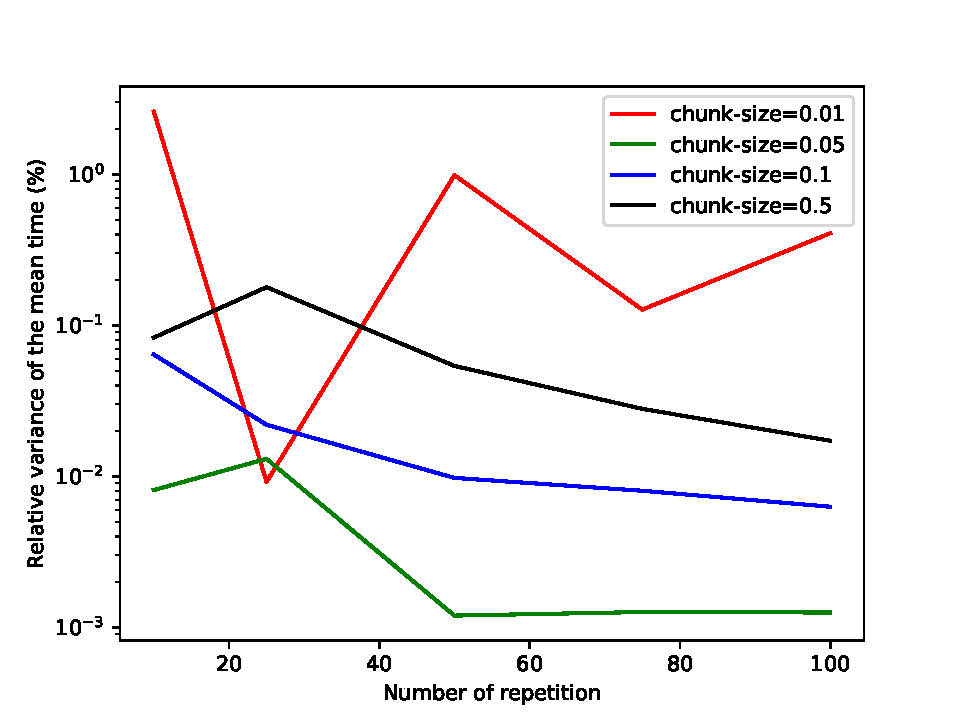
\includegraphics[width=\textwidth]{images/relvar_100_8.pdf}
		\caption[]%
		{{\small 100$\times$100 on 8 threads}}    
	\end{subfigure}
	\quad
	\begin{subfigure}[b]{0.475\textwidth}   
		\centering 
		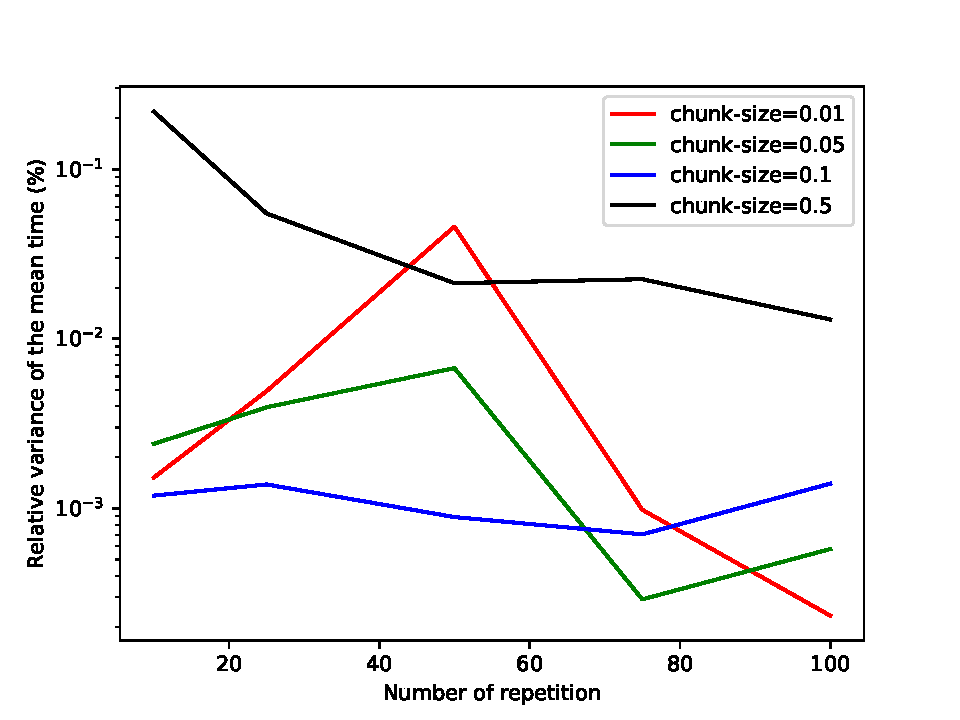
\includegraphics[width=\textwidth]{images/relvar_500_8.pdf}
		\caption[]%
		{{\small 500$\times$500 on 8 threads}}    
\end{subfigure}
	\caption[Standard deviations]
	{\small Variances of the mean of execution times for different experiments  and different chunk sizes on Matrix Multiplication algorithm} 

\end{figure*}
\newpage
Figure 2 shows that in most cases for a 100x100 matrix the variance of the mean get smaller when $N_{rep}$ get bigger which ultimately means that the more repetitions you do when generating your data, the more accurate your execution time measurement becomes. There are oscillations in some cases, mostly with 500x500 matrices, but the relative variances is always smaller or close to 1\% (the maximal relative variance measure was 2\%). Since the relative variance is always smaller or close to 1\%,even for 10 repetitions, it was decided that 10 repetitions would be enough for this work. This means that every time I run any experiment, I measure the execution time of a HPX for-loop 10 times and output the mean. This choice was made to accelerate the data generation process but a larger number of repetitions can be used to generate more precise data at the cost of time.

\subsubsection{Variations of optimal chunk size for a given experiment}

Now that it has been demonstrated that you can accurately measure execution time by having more and more repetitions, one would expect the optimal chunk size to be the same each time you run the same experiment. This is important because the goal of the project is to predict the optimal chunk-size based on the features of a loop. If you run an experiment twice and get different optimal chunk sizes, than it would mean that there is no function $$f:\{X_i\} \rightarrow cs_i$$ 

 . It is important to be sure that such a function can exist because this is the function that will be approximated with machine learning. To analyze the variations in optimal chunk size, the same experiments as previous section have been run. Chunk sizes of \{0.01,0.05,0.1,0.5\} have once again been used on loops with 100 and 500 iterations with 2,4 and 8 threads. Here are the optimal chunk sizes for each experiment. Each column represents an experiment and each row represents a repetition on the given experiment.
\begin{table}[H]
	\centering
	\caption{Optimal Chunk size for repetitions of matrix multiplication experiments}
	\label{my-label}
	\begin{tabular}{|c|c|c|c|c|c|c|}
		\hline
		&
		\multicolumn{2}{|c|}{2 Threads} & \multicolumn{2}{c|}{4 Threads} & \multicolumn{2}{c|}{8 Threads} \\ \hline
		experiment&100x100       & 500x500       & 100x100       & 500x500      & 100x100       & 500x500      \\ \hline
		1&0.5            & 0.5            & 0.5            & 0.01          & 0.05           & 0.5           \\ \hline
		2&0.5            & 0.5            & 0.1            & 0.05          & 0.05           & 0.05          \\ \hline
		3&0.5            & 0.5            & 0.1            & 0.05          & 0.05           & 0.5           \\ \hline
		4&0.5            & 0.5            & 0.1            & 0.05          & 0.01           & 0.01          \\ \hline
		5&0.5            & 0.5            & 0.1            & 0.05          & 0.05           & 0.01          \\ \hline
		6&0.5            & 0.5            & 0.1            & 0.05          & 0.05           & 0.01          \\ \hline
		7&0.5            & 0.5            & 0.1            & 0.05          & 0.05           & 0.01          \\ \hline
		8&0.5            & 0.5            & 0.5            & 0.05          & 0.05           & 0.01          \\ \hline
		9&0.5            & 0.5            & 0.1            & 0.01          & 0.01           & 0.01          \\ \hline
		10&0.5            & 0.5            & 0.1            & 0.5           & 0.05           & 0.01          \\ \hline
	\end{tabular}
\end{table}

Table 1 shows some variations in optimal chunk size when you run the same experiment different times and therefore we are not guaranteed to find the same target values when re-generating data. However, for these tests, we can clearly identify a value for chunk size that is selected more often than the other values. To conclude, the function $f$ does seem to exist but with some background noise.

\subsubsection{Comparison of executions times for all chunk size candidates}
As seen previously, when you run the same experiment multiple times, there is some variation in the optimal chunk size obtained. To understand this in more details, I decided to analyze the variations of execution times with respect to different chunk size candidates.
 In fact, for experiments where there is very little variations in executions times for different chunk-sizes, we should expect huge variations in optimal chunk-size since the times are so close that the optimal chunk size keeps changing.

One way to study the variations between execution times for different chunk sizes is the variance. Here the variance is calculated by the following for an experiment $i$:
$$\operatorname{VAR}(t_i)=\frac{1}{Card(CS)-1}\sum_{cs \in CS}(t(X_i,cs)-\bar{t}_i)^2$$
with 
$$\bar{t}_i=\frac{1}{Card(CS)}\sum_{cs \in CS}t(X_i,cs)$$

 $Card(CS)$ is the cardinality of the set $CS$ which means how many candidates are being tested. Also, in that case the mean $\bar{t}_i$ is the average of executions times between all chunk sizes candidates. This variance can be interpreted as how much chunk size affect the execution time of a loop overall. Small values of variance mean that there is no significant impact on execution times and a huge variance means that you really need to find the right chunk size.

The variance has been calculated on a Matrix Multiplication algorithm with 100,200,300,400, 500,600,700,800 iterations and 1,2,4,6,8,10,12,14 threads and $CS=\{0.01;0.05;0.1;0.5\}$
Here the variance is shown using a color map.

\begin{figure}[H]
	\centering
	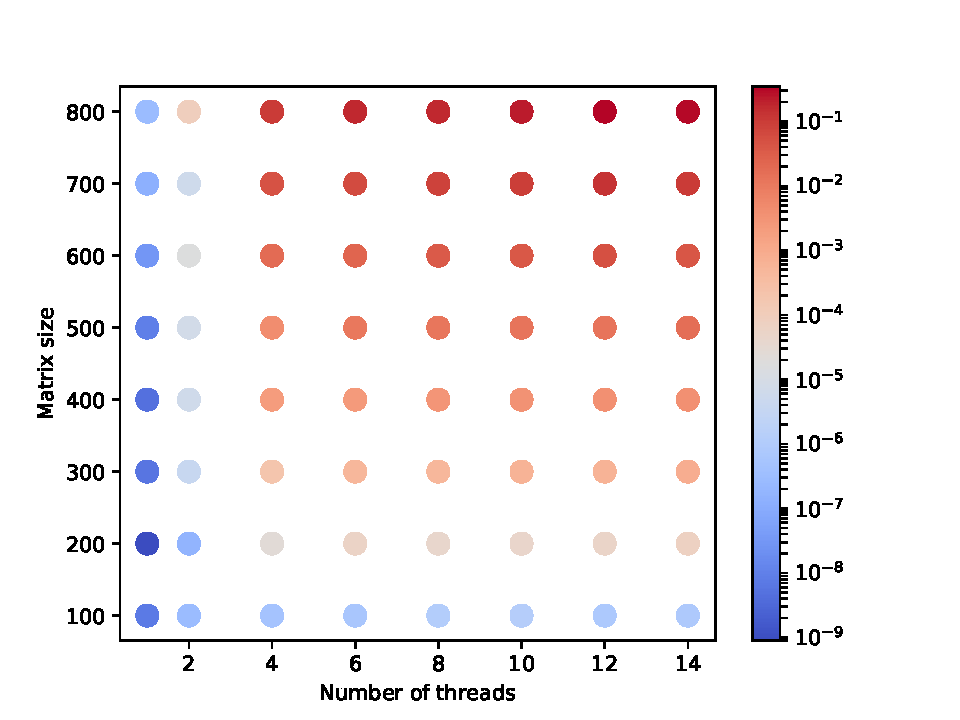
\includegraphics[width=100mm]{images/var_chunk_sizes.pdf}
	\caption{Variance of execution times as a function of features on Matrix Multiplication algorithm}
\end{figure}

 Figure 3 shows that when you add more threads and more iterations, the more variations you observe when measuring execution time for different chunk-sizes. However there is a problem with this result, the execution times are not all on the same scale. In fact the more iterations you have, the bigger the execution time. In that case, the execution time ranges from 0.005 to 2 seconds depending on the experiment. To solve this problem, the relative variance must once again be used. 

Here is a plot of the relative variance for all the same experiments:

\begin{figure}[H]
	\centering
	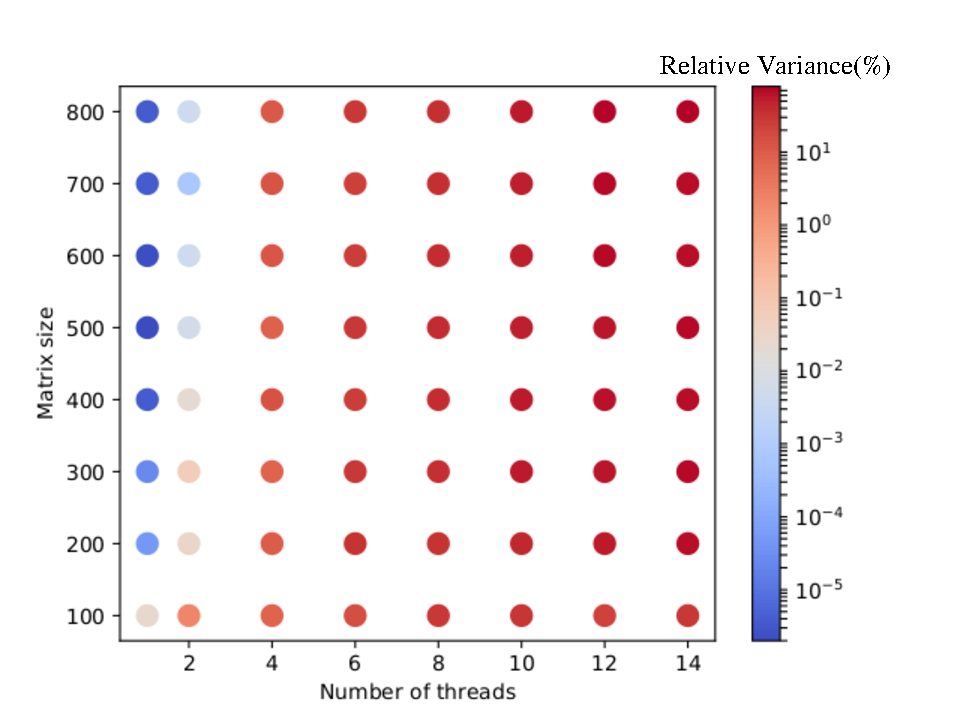
\includegraphics[width=100mm]{images/rel_var_chunk_sizes.pdf}
	\caption{Relative Variance (\%) of execution times as a function of features on Matrix Multiplication algorithm}
\end{figure}

Figure 4 shows that the relative variance depends highly on the number of threads. It appears that the lowest variance is obtained when using only one threads which makes sense since 1 thread is equivalent to sequential execution. Therefore, it has been decided that the number of threads would never be put to 1 because of the low relative variance between execution times. We can also see that by adding more threads, we add more variances in the execution times because an efficient use of these threads results in a significantly smaller execution time.

\subsubsection{Function analysis}
In this section, the focus will be on analyzing the function that will be approximated by machine learning

$$f:\{X_i\} \rightarrow cs_i$$

The data used to visualize this function is comprised 64 experiments of matrix multiplication with 100,200,300,400, 500,600,700,800 iterations and 1,2,4,6,8,10,12,14 threads. The chunk sizes candidates were $CS=\{0.005; 0.01 ;0.05; 0.1; 0.2; 0.5\}$

First of all, it is important to note that since when generating data with only a matrix multiplication function, the features <Number of Operations> <Number of Float Operations> and <Number of Comparison Operations> are a polynomial function of <Number of Iterations>

This means that of all 6 features, only 2 can be used (Deepest loop level is not necessary because it is the same for each matrix multiplication experiment). Here is a punctual color-map of the function with the current data.

\begin{figure}[H]
	\centering
	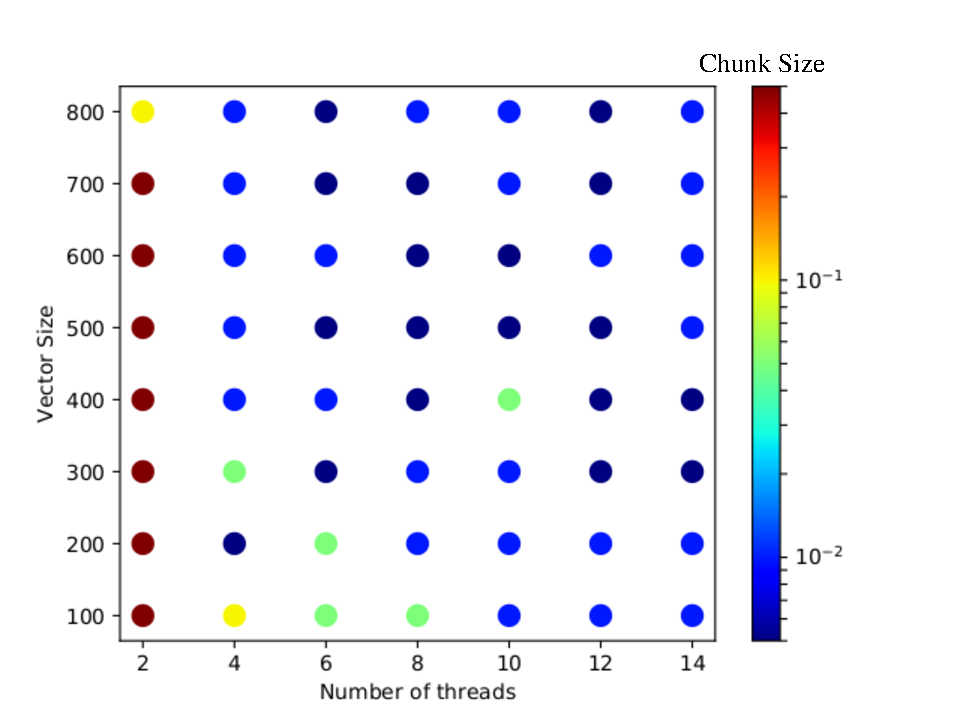
\includegraphics[width=120mm]{images/chunk_size_function_matrix.pdf}
	\caption{Optimal chunk size as a function of features on Matrix Multiplication algorithm}
\end{figure}

Figure 5 shows that the number of threads has an impact on optimal chunk size For 100 iterations where we can see a steady decrease of chunk size with respect to number of treads. However for bigger matrices, the function oscillates. These oscillations are caused by the fact that execution times between 0.005 and 0.01 are very close. Here is a table of some execution times to show my point. (Note 0.2 was removed because it was never selected)

\begin{table}[h]
	\centering
	\caption{Execution times for 5 experiments of Matrix multiplication}
	\label{my-label}
	\begin{tabular}{|c|c|c|c|c|c|}
		\hline
		chunk size&0.005& 0.01           & 0.05 & 0.1 & 0.5 \\ \hline
		experiment 1&0.221386 & 0.219532  & 0.247906    & 0.253246        & 0.629754 \\ \hline
		experiment 2&0.229569 & 0.229047 & 0.238892   & 0.422549        & 1.02871  \\ \hline
		experiment 3&0.168765 & 0.166738  & 0.2141   & 0.4157       & 1.0294  \\ \hline
		experiment 4&0.122448 & 0.121981  & 0.136015    & 0.260424        & 0.709034 \\ \hline
		experiment 5 &0.0179531 & 0.0177467 & 0.0181951  & 0.0337951        & 0.082139 \\ \hline
	\end{tabular}
\end{table}

Table 2 shows that in all experiments, the execution times for 0.01 and 0.005 are very close. In fact the relative difference is around $1\%$ in average. The oscillations are caused by the fact that the time difference between 0.005 and 0.01 is smaller than the noise.

Here are some way we try to remove the oscillations

1-Matrices size is too small and therefore execution times for certain chunk sizes are too close to be reliably distinguishable.

2-There is a missing dynamic feature that is causing the variations which seem uncorrelated to the 2 current features.

3- Some chunk size candidates are too close to be reliably distinguished so the choice of candidates could be optimized.
\
\subsubsection{First approach}

The first approach was to use bigger matrices of sizes:
100,200,400,600,800,1000,1500,
2000,2500 with chunk-size candidates $CS=\{0.0005;0.001; 0.005; 0.01; 0.05; 0.1;0.5\}$

\begin{figure}[H]
	\centering
	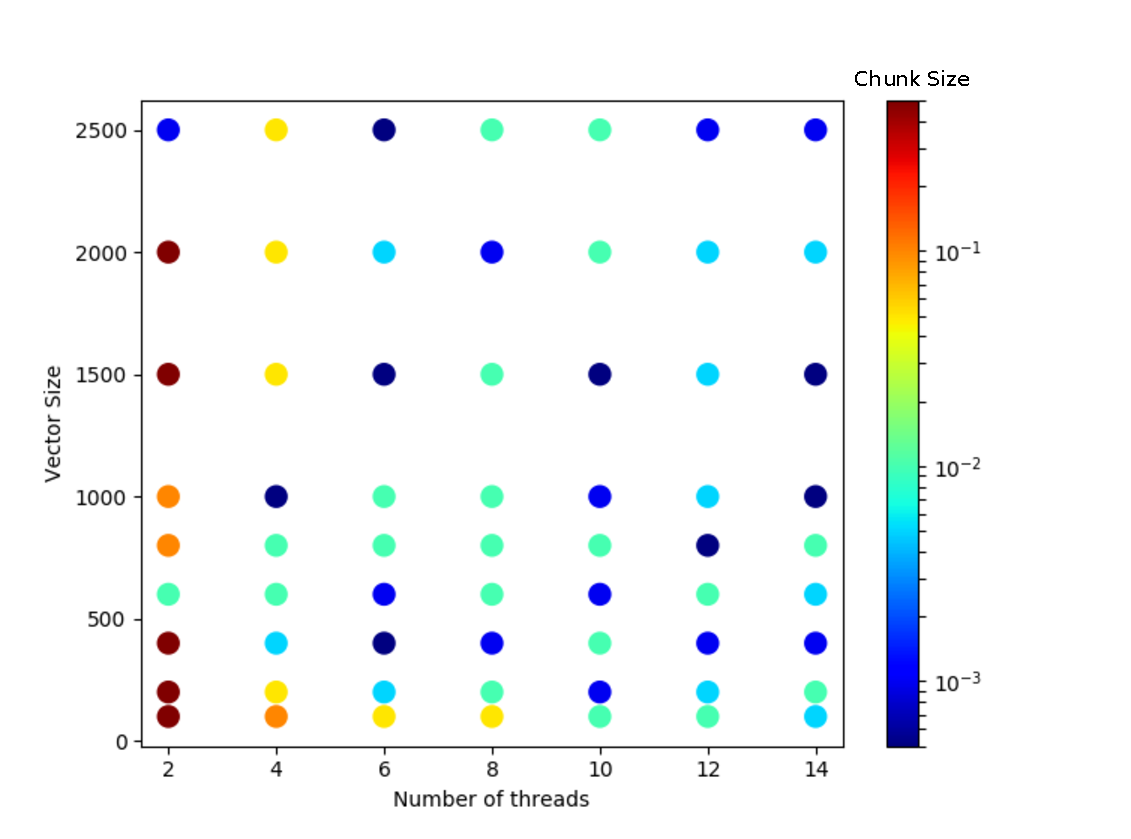
\includegraphics[width=120mm]{images/chunk_size_function_matrix_big.pdf}
	\caption{Optimal Chunk Size as a function of features on Matrix Multiplication algorithm with bigger matrices}
\end{figure}

In figure 6, we still observe oscillations so I decided to examine the execution times once more.

\begin{table}[h]
	\centering
	\caption{Execution times for 1000x1000, 1500x1500, 2000x2000 and 2500x2500 Matrices}
	\label{my-label}
	\begin{tabular}{|c|c|c|c|c|c|c|c|}
		\hline
		chunk size&0.0005  & 0.001   & 0.005   & 0.01    & 0.05    & 0.1     & 0.5     \\ \hline
		experiment 1&NaN     & 1.06075 & 1.10638 & 1.01317 & 1.13454 & 1.15139 & 3.35216 \\ \hline
		experiment 2&NaN     & 3.33313 & 3.34309 & 3.33242 & 3.88524 & 3.93604 & 9.56364 \\ \hline
		experiment 3&7.91752 & 7.84541 & 7.8376  & 7.88513 & 9.22963 & 9.44594 & 22.4268 \\ \hline
		experiment 4& 15.4564 & 15.5674 & 15.4928 & 15.4807 & 18.0824 & 18.2549 & 43.5778 \\ \hline
	\end{tabular}
\end{table}

According to Table 3 it appears like once again, the execution times for the smaller chunk-sizes are very close, which explains the oscillations in the function. Having bigger matrices didn't seem to solve the issue.

\subsubsection{Second approach}

The idea would be to add the idle rate of the CPU's as a dynamic feature in the hope of having a better function.
This hasn't been done yet.

\subsubsection{Third approach}
By looking at Table 2 and Table 3, it seems that chunk sizes which are different by a factor of two give very similar execution times while chunk sizes with a factor of 5 or more gave bigger differences. Here I will try to have a set of chunk size candidates where all consecutive chunk sizes are separated by the same multiplicative factor. First let's try with a factor 4. $CS=\{0.5;0.125;0.03125;0.0078125;0.001953125\}$. This means that the job will be split into 2,8,32,128,512 chunks.

Here is for small matrices

\begin{figure}[H]
	\centering
	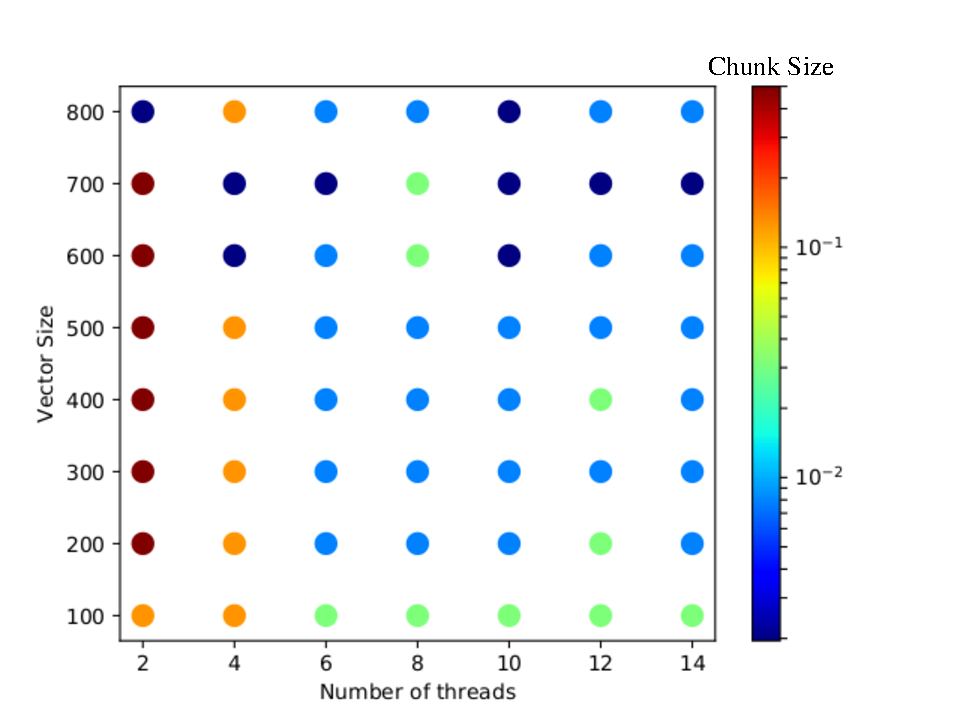
\includegraphics[width=120mm]{images/chunk_size_function_matrix_uniform_log.pdf}
	\caption{Optimal Chunk Size as a function of features with chunk sizes candidates uniform on logscale}
\end{figure}

And for bigger matrices
\begin{figure}[H]
	\centering
	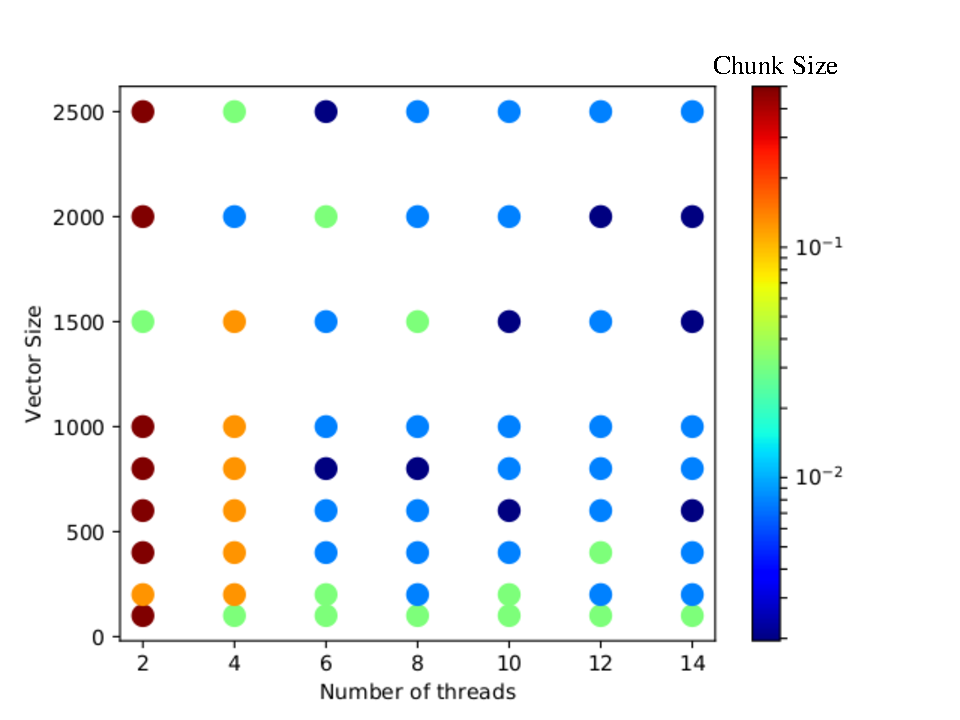
\includegraphics[width=120mm]{images/chunk_size_function_matrix_uniform_log_big.pdf}
	\caption{Optimal Chunk Size as a function of features on bigger matrices with chunk sizes candidates uniform on logscale }
\end{figure}

Figure 7 and Figure 8 are very encouraging, We can see some reduction of the oscillations. The choice of candidates is still not optimal but we can see that choosing candidates is really important. Here is the results with 50 repetitions

\begin{figure}[H]
	\centering
	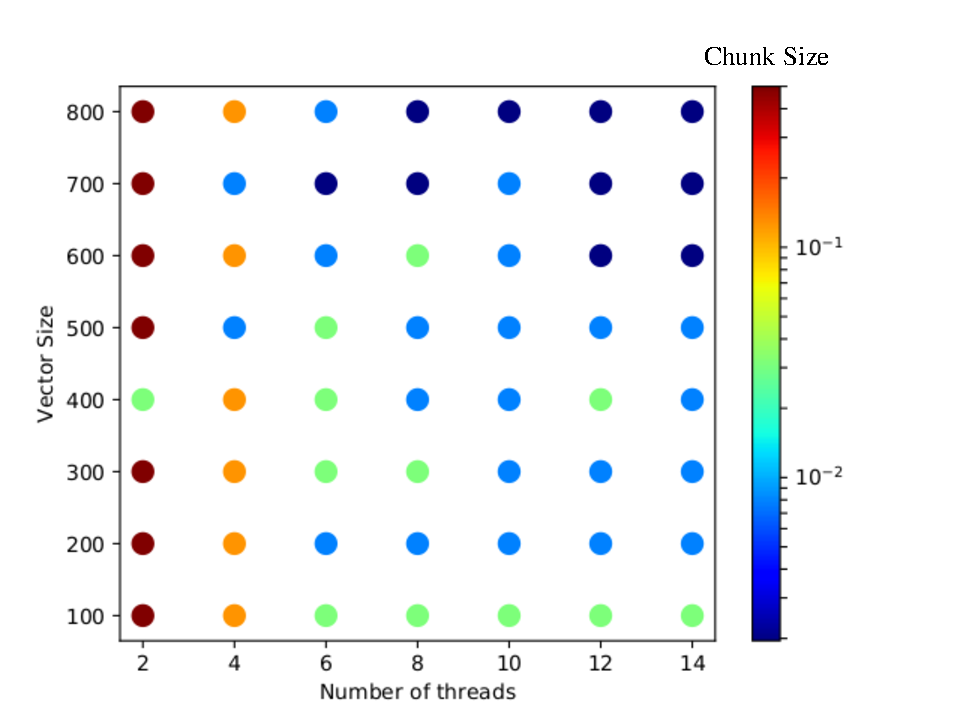
\includegraphics[width=120mm]{images/chunk_size_function_matrix_uniform_log_50rep.pdf}
	\caption{Optimal Chunk Size as a function of features with chunk sizes candidates uniform on logscale and 50 repetitions}
\end{figure}

Figure 9 is closer to what you would expect, the more threads and the bigger the Matrix, the more advantageous it becomes to split your job in many chunks. There is still some noise but it is unavoidable at this point. At least we can reduce it by changing the set of candidates.
\subsection{1D Stencil algorithm}

Another algorithm that was studied individually was 1D Stencil algorithm. It was studied because of its simplicity which make it different from Matrix Multiplication. In the stencil algorithms, you have a vector $\vec{x} \in \mathbb{R}^N$ and you apply $x_i=0.5x_{i-1}+x_i+0,5x_{i+1} \forall i=1,2,3...N-1$. To make this algorithm parallelizable, the output must be stored in a new vector.

Here the features <input size> can be renamed <vector size> since the 1D stencil is applied on a vector.
\newpage
\subsubsection{Function Analysis}

\begin{figure*}[h]
	\centering
	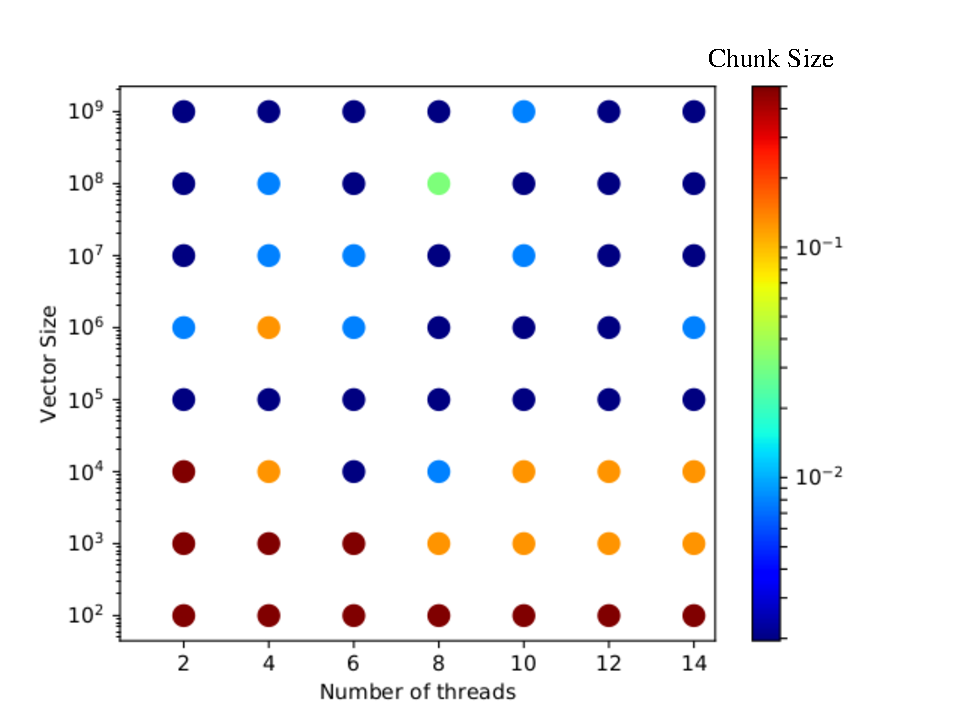
\includegraphics[scale=0.8]{images/stencil_function.pdf}
	\caption{Optimal Chunk Size as a function of features on Stencil algorithm with chunk sizes candidates uniform on logscale}
\end{figure*}
Figure 10 is very interesting because we really see a different behavior than with matrix Multiplication. Here the number of threads doesn't seem to have the same impact as Vector size which is the opposite of what was observed previously.

\newpage
\subsection{Data Set with many functions}
In this section, the focus will be on a bigger data set which is comprised of 278 experiments with many lambda functions. Here is a descriptions of all the functions used:



\begin{table}[h]
	\begin{tabular}{|c|c|c|}
		\hline
		\textbf{Name} & \textbf{Description} & \textbf{Numbers of iterations} \\ \hline
		Nothing() & Does Nothing & 10\textasciicircum{}7 \\ \hline
		Swap() & Swap elements between two vectors & \begin{tabular}[c]{@{}c@{}}100,1000,10000\\ 100000,100000\end{tabular} \\ \hline
		Stream() & Basic stream algorithm & 1000,10000,100000 \\ \hline
		Matrix\_Vector\_Mult() & Matrix Vector multiplication & \begin{tabular}[c]{@{}c@{}}100,500,1000\\ 5000,10000,20000\end{tabular} \\ \hline
		Dyadic() & Applies a dyadic product on two vectors & 100,1000,10000 \\ \hline
		Cosine() & \begin{tabular}[c]{@{}c@{}}Applies a cosine function on \\ each element of a given\\  vector using Taylor series\end{tabular} & \begin{tabular}[c]{@{}c@{}}100,1000,10000\\ 100000\end{tabular} \\ \hline
		Matrix\_Matrix\_Mult() & Matrix Matrix multiplication & \begin{tabular}[c]{@{}c@{}}100,500,1000,\\ 1500,2000,2500\end{tabular} \\ \hline
		Max() & \begin{tabular}[c]{@{}c@{}}Find the max of each column of a \\ 3 dimensional array\end{tabular} & \begin{tabular}[c]{@{}c@{}}1000,5000,10000,\\ 50000,100000\end{tabular} \\ \hline
		Tensor\_Generator() & Generates a tensor of dimension 4 & 100,200 \\ \hline
	\end{tabular}
	\caption{All functions used to generate 278 experiments}
\end{table}

Due to the difficulty of analyzing functions of more than 2-3 dimensions, this function has not been analyzed yet. However at some point it should be analyzed as this data-set is closer to what will be used in practice.

\section{Machine-Learning}

\subsection{Classification or Regression}
In machine learning there are two type of functions approximators, classifications and regressions. Classification can output any value from a finite set and this method was previously used with $CS=\{0.001;0.01;0.1;0.5\}.$ Regression can output any number from a infinite set of candidates so it can be seen as classification algorithm where the number of candidates grows to infinity. But one has to wonder, Is it better to use less or more chunk sizes candidates. In [0] chunk sizes of $\{0.01;0.01;0.1;0.5\}$ have proven to be successful but can we improve performance by adding more candidates? If the variance of time is null than we have:

$$CS \subset CS' \Rightarrow \underset{cs \in CS'}{\min}t(X_i,cs)\leq \underset{cs \in CS}{\min}t(X_i,cs) \, \, \forall i$$

Which is to say that adding new candidates should always give a smaller or equal minimum of time. However, as seen earlier, there is variance in time measurement but we can hope that the variance is small enough to ensure that the statement is still true. This is my main hypothesis that will be tested:\\

HYPOTHESIS: Adding more candidates to $CS$ will reduce the execution times of hpx-loops.


 One way to test this assertion is to try a classification algorithm and adding more than 4 candidates but this becomes unpractical as generating data for many candidates takes longer. As an example data with 8 candidates takes around twice as long to generate as data with 4 candidates. Also, classification algorithms tends to reduce in accuracy the more candidates you add. However, if a regression algorithm is used, we technically have a set $CS$ which is infinite, even if we only use  4 or 5 candidates in the training set. This is because regression can interpolate between two candidates. For example if the candidates used when training are $\{0.01;0.1;0.5\}$ a regression could output any value in between like 0.0245879097 or 0.3333453 instead of being restricted to the finite set $\{0.01;0.1;0.5\}$.
 So let me rephrase the hypothesis:
 
 HYPOTHESIS(rephrase): Using a regression algorithms will give smaller execution times than classification algorithms.
 
  The goal of this analysis will be to confirm or infirm this hypothesis.


\subsection{Matrix Multiplication data-set}

The 4 regression algorithms that were studied on the matrix multiplication data-set are Support Vector Regression, Neural Network Regression, k-Nearest-Neighbors Regression and Random Forest Regression. To compare the performance of these algorithms, the k-fold cross validation has been used. In this method, you divide your data-set into k subsets and than you train the regression on (k-1) subsets and use the last subset as a testing set on which the regression will be evaluated. The measure of the error will be done by scikit's $MeanSquaredError()$ which outputs the mean of the squared error between the test subset and the predictions.

$$MSE(\hat{f})=\frac{1}{N_\text{test}}\sum_{i=1}^{N_\text{test}}(y_i-\hat{f}(X_i))^2$$

Where $\hat{f}$ represent the regression function which is an approximation of $f$, $X_i$ represent the features for an experiment $i$, $cs_i$ represents the target values and $N_{test}$ represents the number of experiments in the test set. It is important to note that to train regression algorithms, you need target values which are on the same scale. To solve this issue a logarithmic scaling is used on the targets values. This means that the error expressed will be the error of the logarithm. This is very hard to visualize but the goal is to compare models so we simply need to compare the errors. The chunk-size is obtained by applying the exponential function to the result of the regression.
Here are some results when using the data used to generate  Figure [5]. A set of 64 experiments of matrix multiplication with sizes of 100,200,300,400, 500,600,700,800 and 2,4,6,8,10,12,14 threads.$CS=\{0.5;0.125;0.03125;0.0078125;0.001953125\}$

\begin{table}[h]
	\centering
	\caption{MSE on 64 experiments of matrix multiplicaition applications with logarithmic scaling using k-fold cross validation}
	\label{my-label}
	\begin{tabular}{|c|c|c|c|c|}
		\hline
		& SVR           & Neural Network & K-Nearest-Neighbors & Random Forest \\ \hline
		k=10 & 1.78+-1.14  & 1.72+-0.91    & 1.28+-1.31        & 1.55+-1. \\ \hline
	\end{tabular}
\end{table}

By using this metric, we can see in Table 5 that the k-Nearest-Neighbors and the Random Forest are the two best algorithms. I believe this is cause by the fact that these functions are piece-wise constant instead of being continuous like SVR and Neural-Network regression. However, the MSE is not a good metric to understand what happens locally when fitting the data. To better understand what happens locally, a graph of Ydata vs Yprediction can be used. In such graphs, cross validation is once again used but now the prediction are outputted. Each color represent a different test set.

\begin{figure}[H]
	\centering
	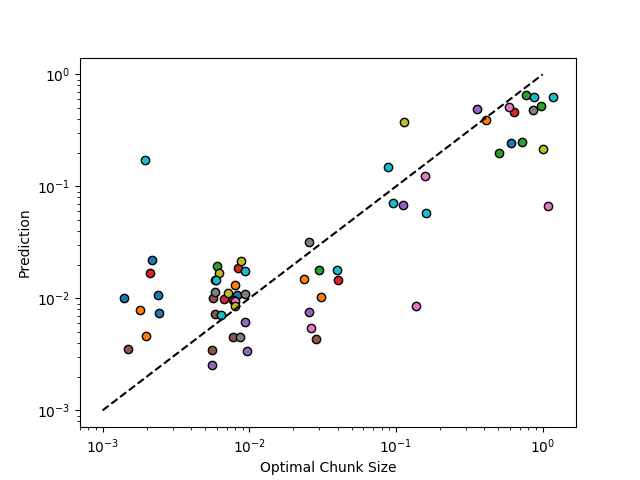
\includegraphics[width=120mm]{images/KNNR_eval.png}
	\caption{k-Nearest-Neighbors predictions vs reality using cross validation with 10 subsets }
\end{figure}

\begin{figure}[H]
	\centering
	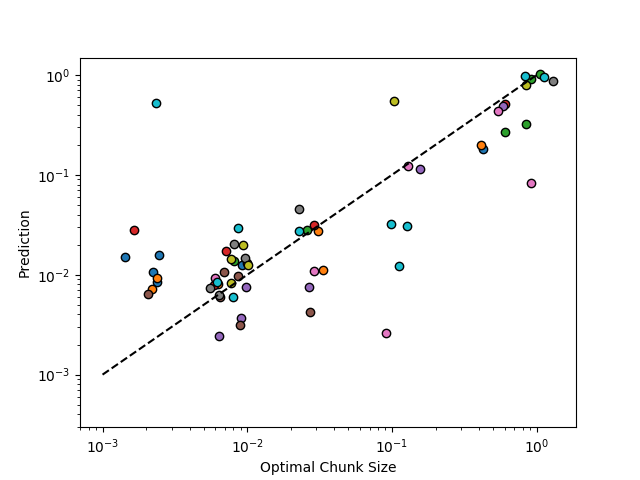
\includegraphics[width=120mm]{images/RFR_eval.png}
	\caption{Random forest predictions vs reality using cross validation with 10 subsets }
\end{figure}

We can see in Figure 11 and Figure 12 that both algorithms are having similar results. However, calculating the error on chunk size is one thing but how does this error translate to execution time? The following measure I will call $Loop\_Total\_Time()$ will be used:

$$Loop\_Total\_time(\hat{f})=\sum_{i=0}^{N_{exp}} t(X_i,\hat{f}(X_i))$$

where $i$ represent a given experiment, $\hat{f}(x_i)$ is the predicted chunk size. $t$ is the execution time of a hpx $for\_each()$ loop with features $X_i$ and using the prediction of the machine learning as chunk size. To make this measure, the predictions on the experiments are obtained in python using k-fold cross validation, then the predictions are used as chunk-sizes on hpx $for\_each$ loops. However, this is an approximation because it doesn't include the time used to make the predictions and because the regressions are not fully implemented in hpx. Even though it's not fully representative of the performance of these algorithms if they were implemented in hpx, this measure is still a useful tool to see if interpolating between chunk-size candidates really improves performances. To verify the hypothesis, 2 regression algorithms were compared to the multinomial classification algorithm which is already fully implemented in hpx. All 3 algorithms are compared to the minimal time which is the summation of all the minimum times for each experiment in the data set.

\begin{table}[h]
	\centering
	\caption{Total execution times (s) on hpx for-loops using the predictions of 3 machine learning algorithms using k-fold cross validation 10 times and comparing with minimal time obtained by taking the minimum time for each experiment on the data-set}
	\label{my-label}
	\begin{tabular}{|c|c|c|c|c|}
		\hline
		& Minimal time &K-Nearest-Neighbors & Random Forest &Multinomial Classification\\ \hline
		k=10 & 9.86
		&10.07+-.16  & 9.95 s+-0.09 & 11.99+-0.4\\ \hline
	\end{tabular}
\end{table}

table 6 shows that both algorithm regression have similar execution times. In fact, the difference between their execution time is lower than the uncertainty of the measurements and therefore we cannot conclude that one is better. However we can see that they both perform better than the Multinomial Classification. 

\begin{figure*}[h]
	\centering
	\begin{subfigure}[b]{0.515\textwidth}
		\centering
		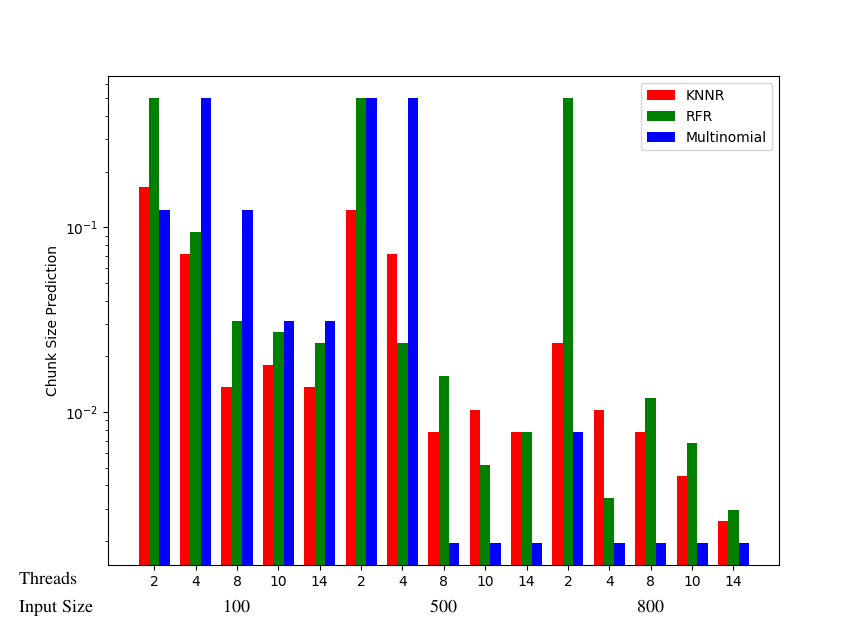
\includegraphics[width=\textwidth]{images/matrix_mult_prediction_bars.png}
		\caption[Network2]%
		{{Chunk sizes}}    
	\end{subfigure}
	\hfill
	\begin{subfigure}[b]{0.475\textwidth}  
		\centering 
		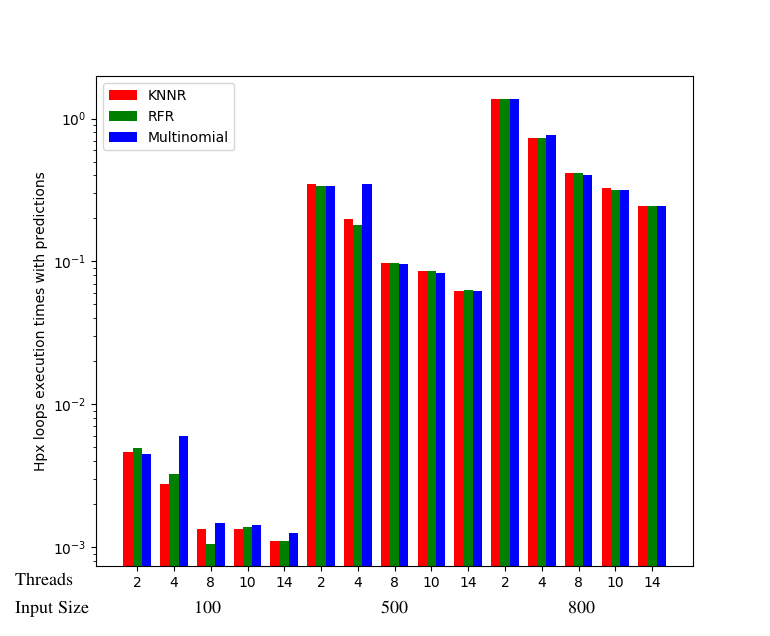
\includegraphics[width=\textwidth]{images/matrix_mult_times_bars.png}
		\caption[]%
		{{HPX loops execution times}}    
	\end{subfigure}
	\caption{Chunk sizes predicted by 3 machine-learning algorithms on Matrix Multiplication functions (a) and the resulting Execution times measured on hpx for-loops (b)} 
	
\end{figure*}



According to Figure 13, it seems that predicts 0.5 on more than 2 threads which never happens with the 2 regressions. This is because the two regressions algorithms take averages in the feature space so they are less likely to predict the highest chunk size 0.5. Predicting 0.5 is very risky because:

$$cs>\frac{1}{\text{number of threads}} \Rightarrow \text{miss-classification error}$$

 When you have $cs>\frac{1}{\text{number of threads}}$, it means that some CPU's are inactive since you don't divide your job into enough chunks to split to all available CPU's. Hence, predicting 0.5 is a high risk because if you are on more than 2 threads, it is a guaranteed error for big algorithms. Since there is less variance on 2 threads, it means that the reward for rightly predicting a  0.5 on 2 threads is smaller than the loss for wrongly predicting a 0.5 on more than 2 threads.
This miss-classification can be manually corrected after the multinomial classification prediction by reducing the chunk size until we have $cs\leq \frac{1}{\text{number of threads}}$. The chunk size obtained may not be the best one, but at least all the CPU's will be active. This will be refereed to as Multinomial Classification corrected.

\begin{table}[h]
	\centering
	\caption{Total execution times (s) on hpx for-loops using the predictions of 3 machine learning algorithms using k-fold cross validation 10 times and comparing with minimal time obtained by taking the minimum time for each experiment on the data-set}
	\label{my-label}
	\begin{tabular}{|c|c|c|c|c|}
		\hline
		& Minimal Time &K-Nearest-Neighbors & Random Forest &Multinomial Class Corrected\\ \hline
		k=10 &9.86 & 10.07+-0.16  & 9.95 s+-0.09 & 10.18+-0.09\\ \hline
	\end{tabular}
\end{table}

\begin{figure*}[h]
	\centering
	\begin{subfigure}[b]{0.5\textwidth}
		\centering
		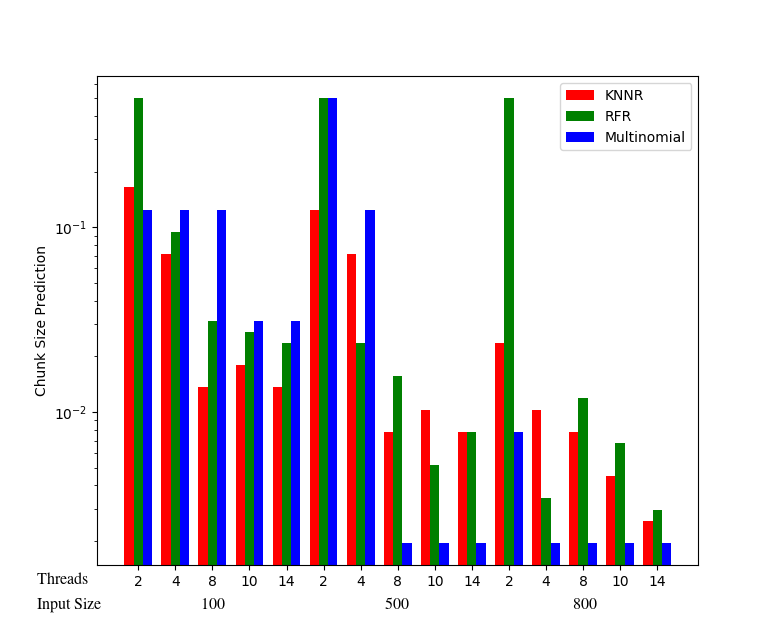
\includegraphics[width=\textwidth]{images/matrix_mult_corrected_predictions_bar.png}
		\caption[Network2]%
		{{Chunk sizes}}    
	\end{subfigure}
	\hfill
	\begin{subfigure}[b]{0.49\textwidth}  
		\centering 
		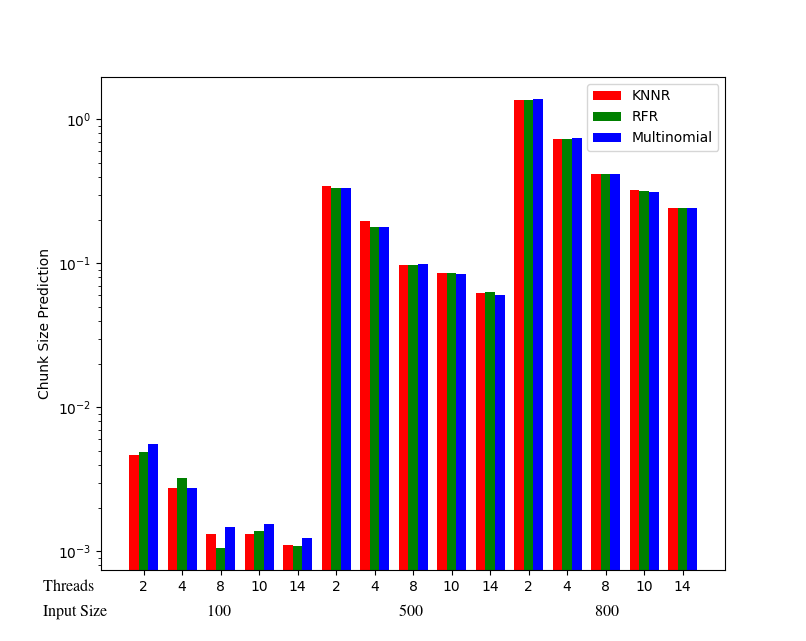
\includegraphics[width=\textwidth]{images/matrix_mult_corrected_times_bar.png}
		\caption[]%
		{{HPX loops execution times}}    
	\end{subfigure}
		\caption{Chunk sizes predicted by 3 machine-learning algorithms on Matrix Multiplication functions (a) and the resulting Execution times measured on hpx for-loops (b)} 
	
\end{figure*}

According to Table 7 and Figure 14, we can note that by manually reducing the aberrant chunk sizes has improved performances but we can still see that the classification has  a longer execution times in some instances. These instance happen to be the ones where the chunk size was manually reduced. However, it cannot be manually reduced any further because we don't know what is the best chunk size. The time difference for these errors is now smaller It is important to note that the color blue is not significant in this graph since its magnitude is around the variance of the data. This can be said because there are blue dots on the doted-line.
\subsection{1D stencil algorithm}
For this function, the multinomial corrected algorithm is compared to the two other regressions:

\begin{table}[h]
	\centering
	\caption{Total execution times (s) on hpx for-loops using the predictions of 3 machine learning algorithms with stencil function using k-fold cross validation 10 times and comparing with minimal time obtained by taking the minimum time for each experiment on the data-set}
	\label{my-label}
	\begin{tabular}{|c|c|c|c|c|}
		\hline
		& Minimal Time &K-Nearest-Neighbors & Random Forest &Multinomial Class Corrected\\ \hline
		k=10 & 93.57&94.65+-2.16  & 95.2 s+-1.98 & 99.32+-3.04\\ \hline
	\end{tabular}
\end{table}
\begin{figure*}[h]
	\centering
	\begin{subfigure}[b]{0.5\textwidth}
		\centering
		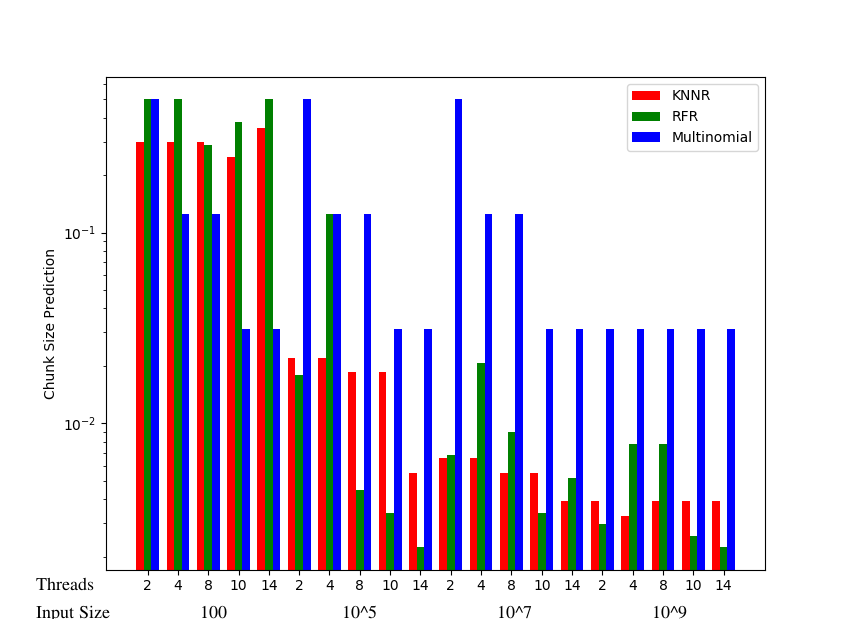
\includegraphics[width=\textwidth]{images/stencil_predictions_bars.png}
		\caption[Network2]%
		{{Chunk sizes}}    
	\end{subfigure}
	\hfill
	\begin{subfigure}[b]{0.49\textwidth}  
		\centering 
		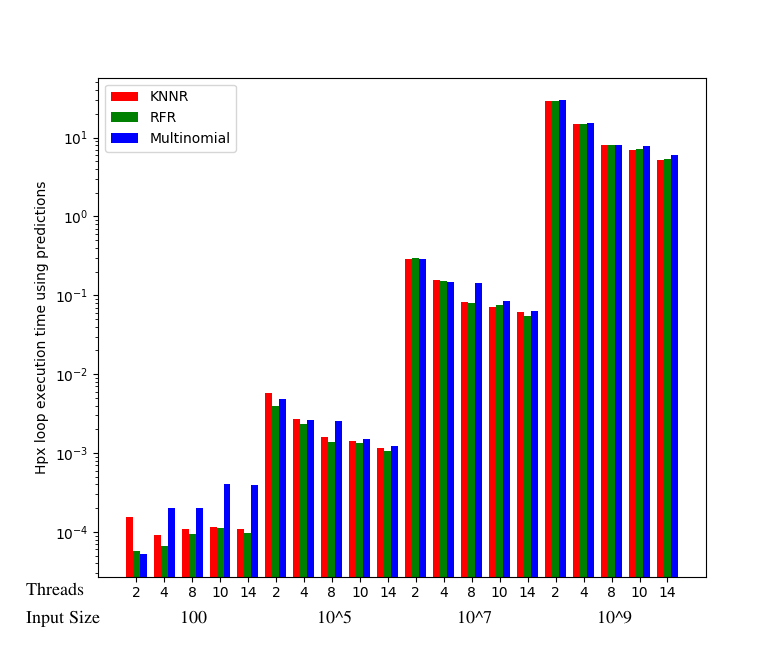
\includegraphics[width=\textwidth]{images/stencil_times_bars.png}
		\caption[]%
		{{HPX loops execution times}}    
	\end{subfigure}
	\caption{Chunk sizes predicted by 3 machine-learning algorithms on Stencil functions (a) and the resulting Execution times measured on hpx for-loops (b)} 
\end{figure*}

Table 8 and Figure 15 both show that Mutinomial CLassification has the bigger total execution times on hpx for-loops.
\subsection{Data Set with multiple functions}

On this data set, the Mean Square Error has once again been measured on the 2 selected regressions:

\begin{table}[h]
	\centering
	\caption{Mean Squared Error on 278 experiments with logarithmic scaling on the chunk sizes candidates using k-fold cross validation 10 times}
	\label{my-label}
	\begin{tabular}{|c|c|c|}
		\hline
		& K-Nearest-Neighbors & Random Forest \\ \hline
		k=10  & 2.18+-1.1        & 1.5+- 0.45 \\ \hline
	\end{tabular}
\end{table}
\begin{figure}[H]
	\centering
	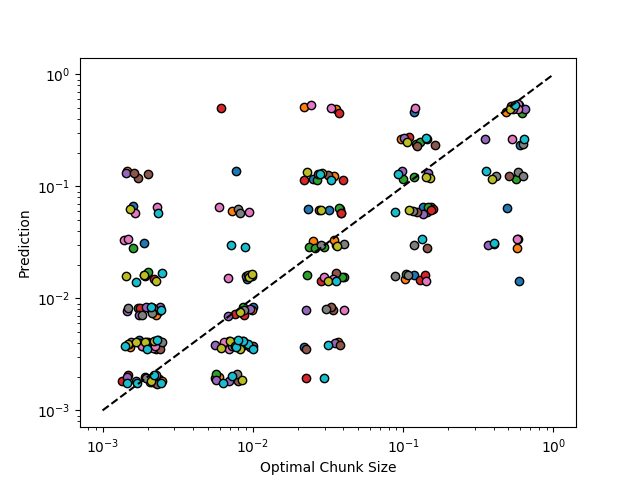
\includegraphics[width=120mm]{images/KNNR_eval_big.png}
	\caption{Evaluation of Nearest-Neighbors with 2 neighbors}
\end{figure}

\begin{figure}[H]
	\centering
	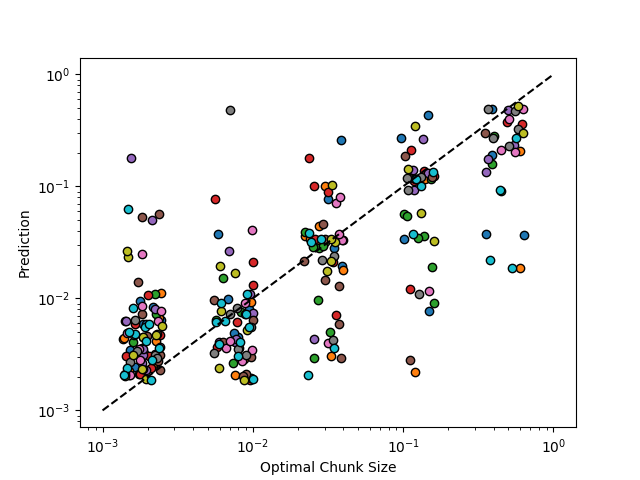
\includegraphics[width=120mm]{images/RFR_eval_big.png}
	\caption{Evaluation of random forest}
\end{figure}

Table 9 shows that k-Nearest-Neighbors has a bigger time on hpx for-loops than Random Forest. I believe it performs worse in that scenario because of the prepossessing on the big data set. In fact not normalizing the features gave a MSE of 1.67. It is normal that kNN is sensible to preprocessing and not RandomForest because it calculates Euclidean distance between points in the feature space. However I have decided to normalize the data nonetheless because the features are on different scales. The exact reason why kNN performs better without normalization could be studied on its own.
\\

Now let's see how this error in prediction relates to execution times. Once again the regressions are compared to Multinomial Classification:


\begin{table}[h]
	\centering
	\caption{Total execution times (s) on hpx for-loops with the predictions of 3 machine learning algorithms on 278 experiments using k-fold cross validation 10 times and comparing with minimal time obtained by taking the minimum time for each experiment on the data-set}
	\label{my-label}
	\begin{tabular}{|c|c|c|c|c|}
		\hline
		& Minimal Time&K-Nearest-Neighbors & Random Forest &Multinomial Class Corrected\\ \hline
		k=10  &312.01&
		 355+-4        & 344+- 4&356+-13 \\ \hline
	\end{tabular}
\end{table}

Like all previous results, Table 10 shows that multinomial classification is worst than the other algorithms. At it point in the project, it was discovered that there was no use of bias inside the multinomial model. The algorithms requires the computation of a linear function $W X$ where $W$ represents the weights which are parameters that need to be optimizes. Adding a bias consist of changing this function to an affine function $WX+b$ where $b$ is called the bias. Let's see how adding a bias improves the results:

\begin{table}[h]
	\centering
	\caption{Total execution times (s) on hpx for-loops with the predictions of 3 machine learning algorithms on 278 experiments using k-fold cross validation 10 times and comparing with minimal time obtained by taking the minimum time for each experiment on the data-set}
	\label{my-label}
	\begin{tabular}{|c|c|c|c|c|}
		\hline
		& Minimal Time&K-Nearest-Neighbors & Random Forest &Multinomial Class Corrected bias\\ \hline
		k=10  &312.01&
		355$\pm$4        & 344$\pm$ 4&341$\pm$4 \\ \hline
	\end{tabular}
\end{table}
In Table 11, we can see that simply adding a bias to the algorithm reduced the execution time on hpx loops by a huge factor. It has now become the best algorithm on the big data set. It may the best on all experiments, but it's still interesting to study the results on each type of function to see if it performs better on all lambda functions:
\newpage
\subsubsection{Nothing}

\begin{table}[h]
	\centering
	\caption{Total execution times (s) on hpx for-loops with the predictions of 3 machine learning algorithms on Nothing function using k-fold cross validation 10 times and comparing with minimal time obtained by taking the minimum time for each experiment on the data-set}
	\label{my-label}
	\begin{tabular}{|c|c|c|c|c|}
		\hline
		& Minimal Time&K-Nearest-Neighbors & Random Forest &Multinomial Class Corrected bias\\ \hline
		k=10  &0.6&
		0.604$\pm$0.021       & 0.6199$\pm$0.025&0.606$\pm$0.025 \\ \hline
	\end{tabular}
\end{table}

\begin{figure*}[h]
	\centering
	\begin{subfigure}[b]{0.5\textwidth}
		\centering
		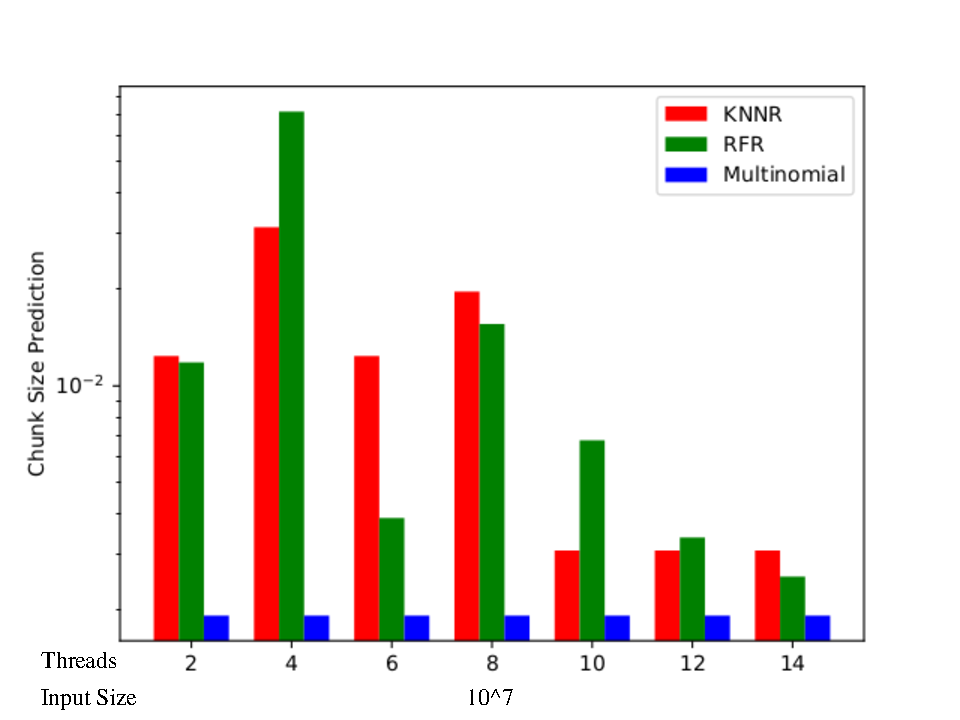
\includegraphics[width=\textwidth]{images/bars_nothing_cs.pdf}
		\caption[Network2]%
		{{Chunk sizes}}    
	\end{subfigure}
	\hfill
	\begin{subfigure}[b]{0.49\textwidth}  
		\centering 
		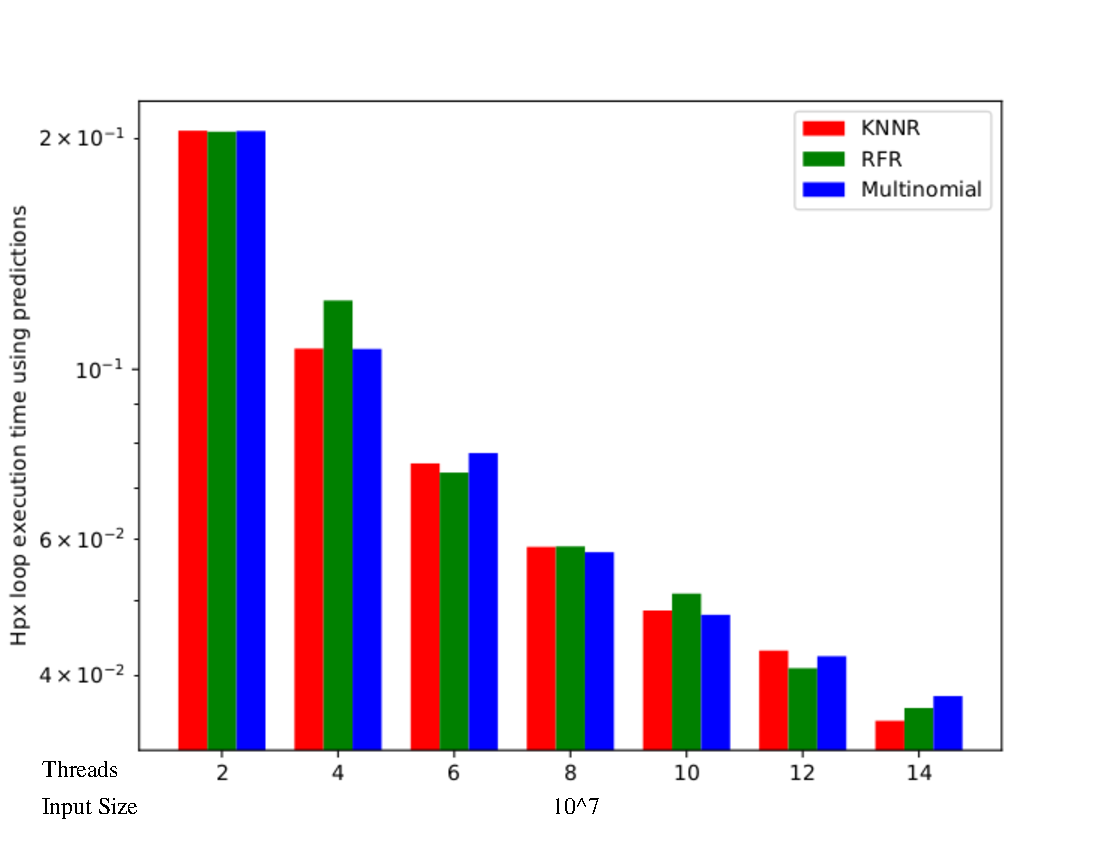
\includegraphics[width=\textwidth]{images/bars_nothing_times.pdf}
		\caption[]%
		{{HPX loops execution times}}    
	\end{subfigure}
	\caption{Chunk sizes predicted by 3 machine-learning algorithms on Nothing functions (a) and the resulting Execution times measured on hpx for-loops (b)} 	
\end{figure*}
Table 12 and Figure 18 show that the results for the 3 algorithms are very close but Random Forest predicted 0.5 on 4 threads which and add a bigger execution time as a result. It is interesting to see that Multinomial Classification always predicts the smallest chunk size. This is because the execution times between $\frac{1}{512}$ and $\frac{1}{128}$ are very close so the algorithm converged too early. This didn't seem to affect that much the total time measured on hpx for-loops.
\newpage
\subsubsection{Swap}

\begin{table}[H]
	\centering
	\caption{Total execution times (s) on hpx for-loops with the predictions of 3 machine learning algorithms on Swap function using k-fold cross validation 10 times and comparing with minimal time obtained by taking the minimum time for each experiment on the data-set}
	\label{my-label}
	\begin{tabular}{|c|c|c|c|c|}
		\hline
		& Minimal Time&K-Nearest-Neighbors & Random Forest &Multinomial Class Corrected bias\\ \hline
		k=10  &0.091&
		0.101$\pm$0.036       & 0.099$\pm$0.036&0.107$\pm$0.037 \\ \hline
	\end{tabular}
\end{table}

\begin{figure*}[h]
	\centering
	\begin{subfigure}[b]{0.5\textwidth}
		\centering
		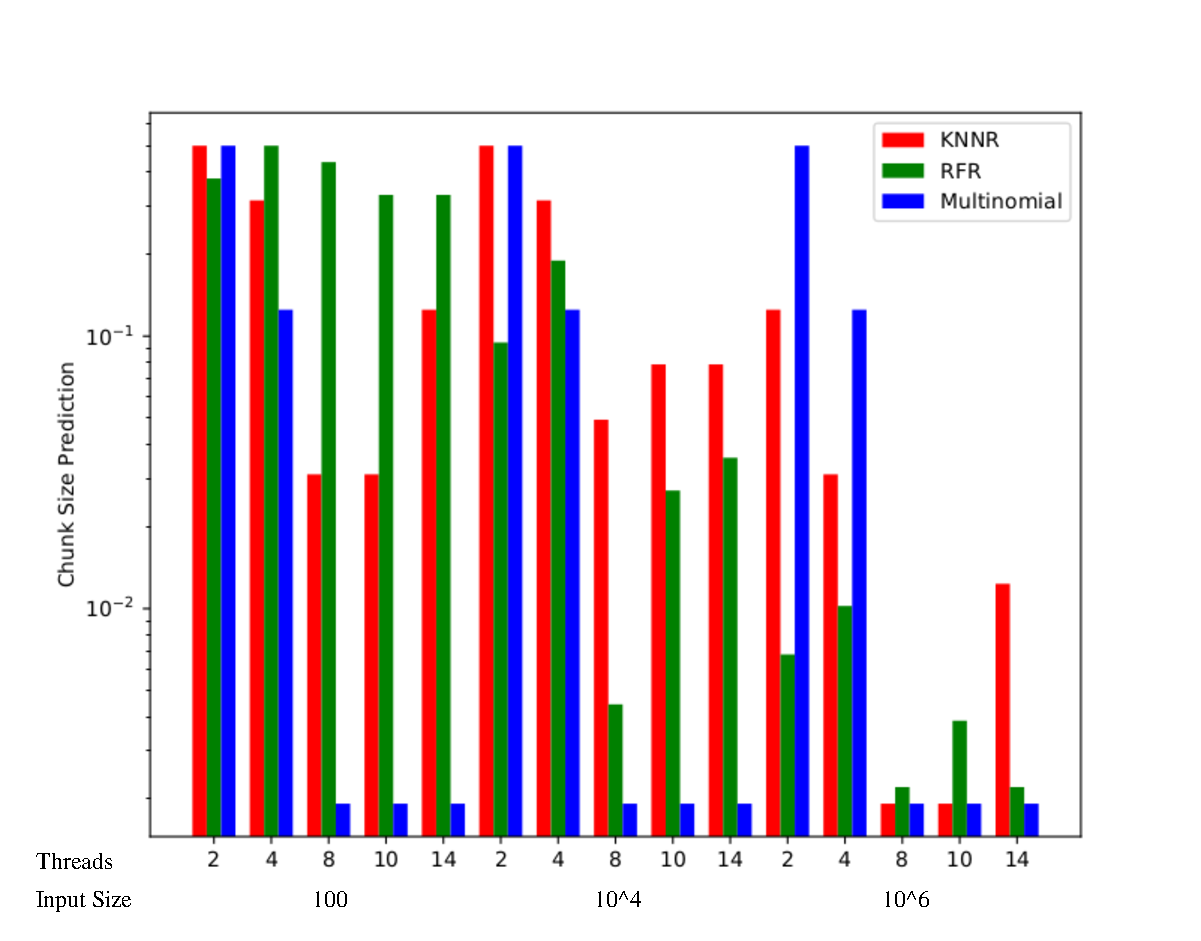
\includegraphics[width=\textwidth]{images/bars_Swap_cs.pdf}
		\caption[Network2]%
		{{Chunk sizes}}    
	\end{subfigure}
	\hfill
	\begin{subfigure}[b]{0.49\textwidth}  
		\centering 
		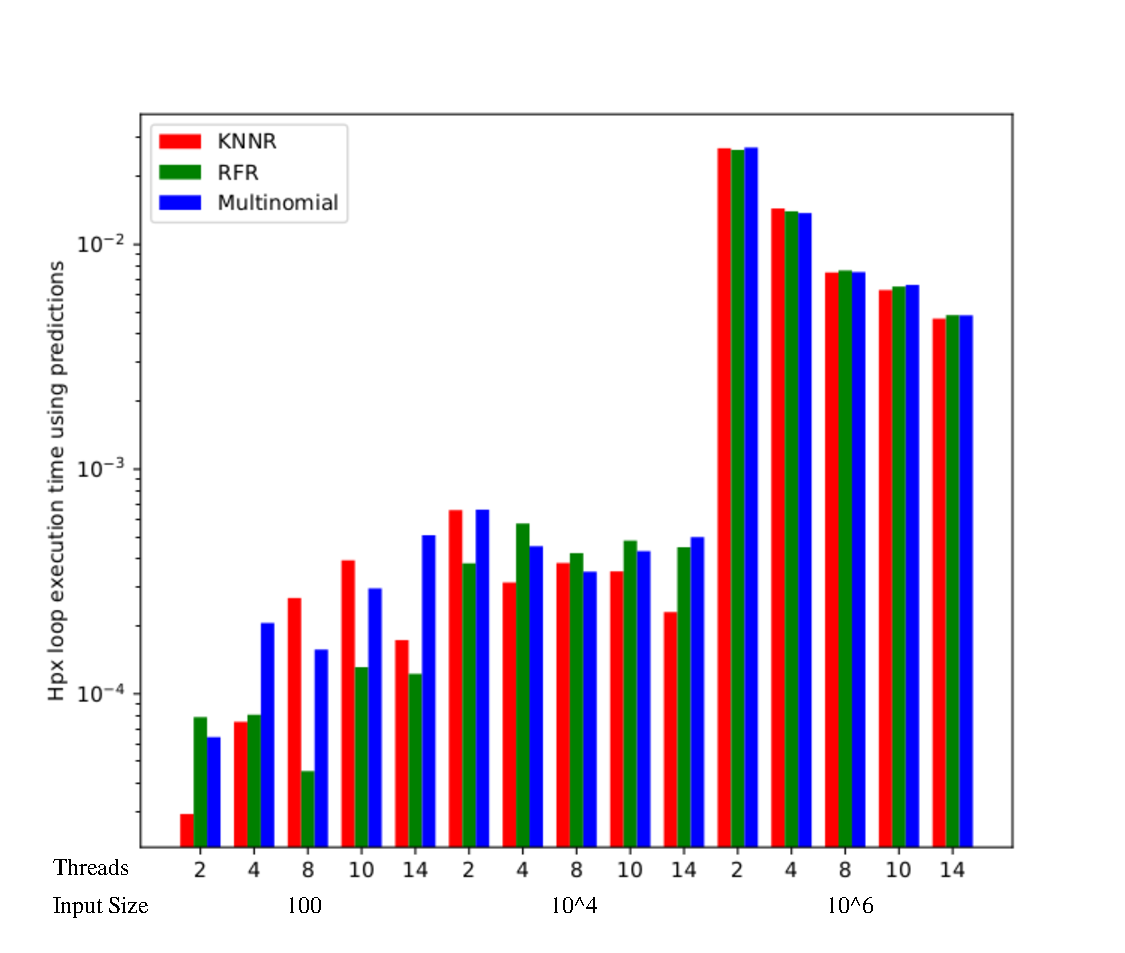
\includegraphics[width=\textwidth]{images/bars_Swap_times.pdf}
		\caption[]%
		{{HPX loops execution times}}    
	\end{subfigure}
	\caption{Chunk sizes predicted by 3 machine-learning algorithms on Swap functions (a) and the resulting Execution times measured on hpx for-loops (b)} 
\end{figure*}
Table 13 and Figure 19 show that times are so close relative to the variance of measurement that it is hard to have conclusions based on these graphs but it seems that the Multinomial algorithm performs worse because it predicts too small chunk sizes which means we observe the overhead of splitting the job.
\newpage
\subsubsection{Matrix-Vector multiplication}

\begin{table}[h]
	\centering
	\caption{Total execution times (s) on hpx for-loops with the predictions of 3 machine learning algorithms on Matrix-Vector multiplication function using k-fold cross validation 10 times and comparing with minimal time obtained by taking the minimum time for each experiment on the data-set}
	\label{my-label}
	\begin{tabular}{|c|c|c|c|c|}
		\hline
		& Minimal Time&K-Nearest-Neighbors & Random Forest &Multinomial Class Corrected bias\\ \hline
		k=10  &3.774&
		3.79$\pm$0.094       & 3.92$\pm$0.062&3.84$\pm$0.1 \\ \hline
	\end{tabular}
\end{table}

\begin{figure*}[h]
	\centering
	\begin{subfigure}[b]{0.5\textwidth}
		\centering
		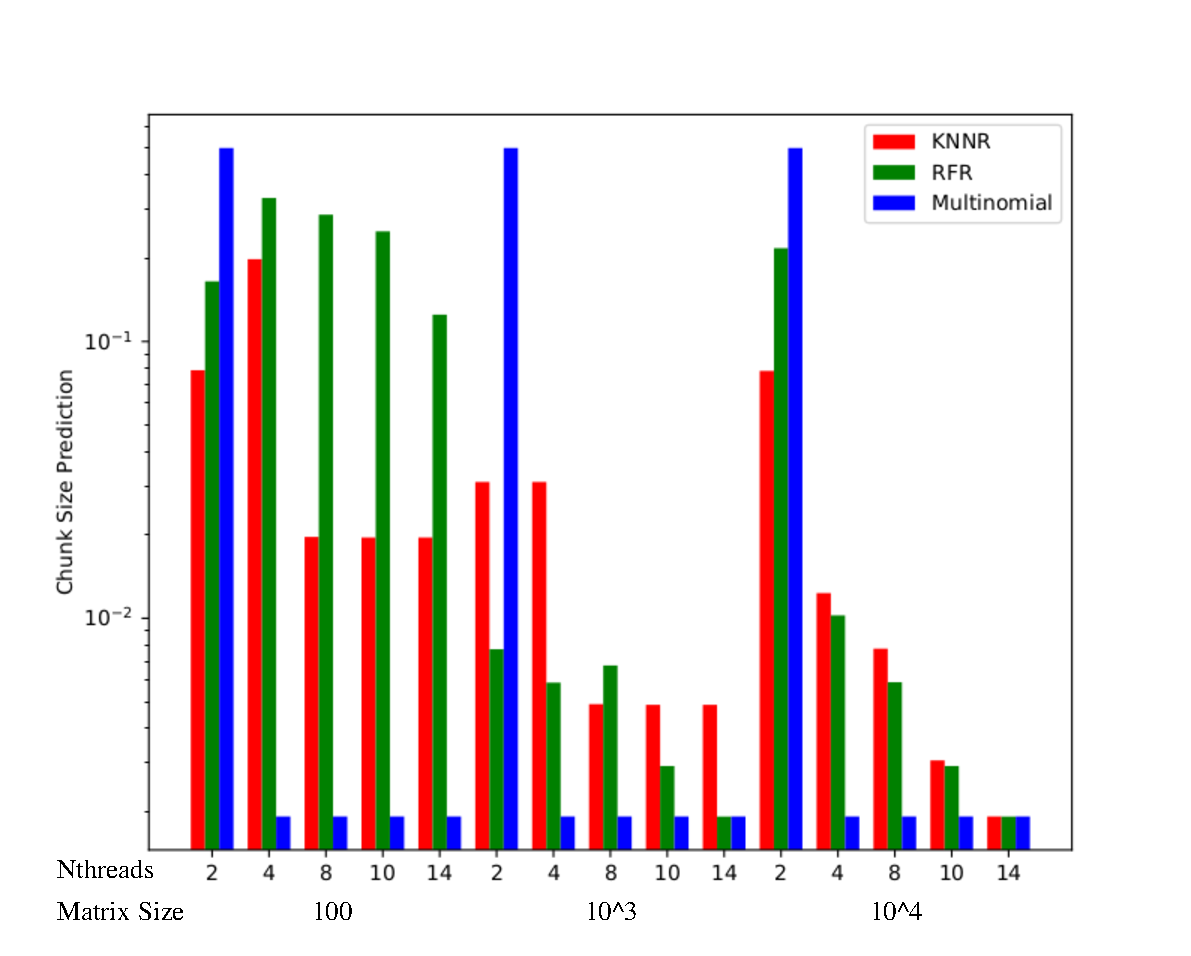
\includegraphics[width=\textwidth]{images/bars_Vector_cs.pdf}
		\caption[Network2]%
		{{Chunk sizes}}    
	\end{subfigure}
	\hfill
	\begin{subfigure}[b]{0.49\textwidth}  
		\centering 
		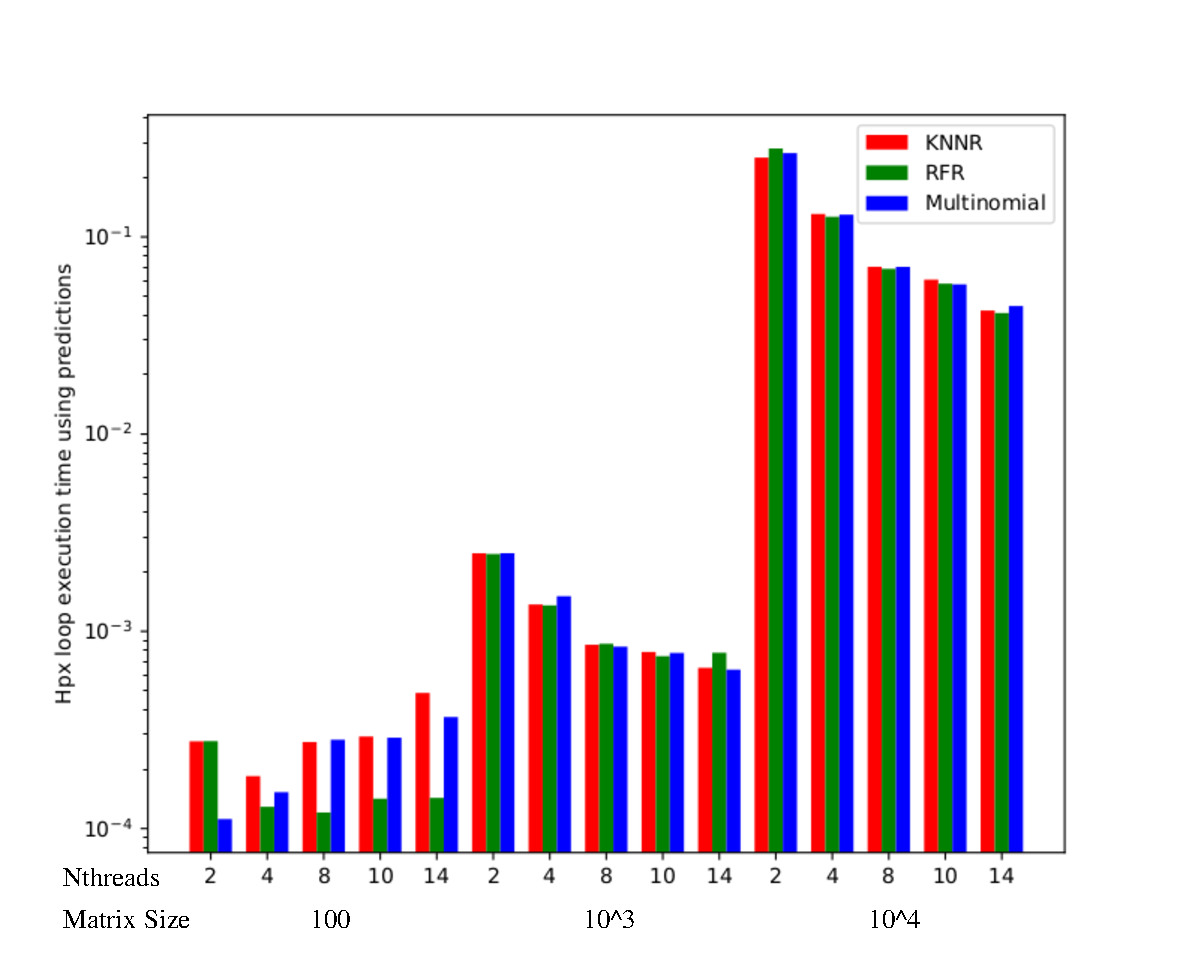
\includegraphics[width=\textwidth]{images/bars_vector_times.pdf}
		\caption[]%
		{{HPX loops execution times}}    
	\end{subfigure}
	\caption{Chunk sizes predicted by 3 machine-learning algorithms on Matrix-Vector multiplication functions (a)and the resulting Execution times measured on hpx for-loops (b)} 
\end{figure*}
Table 14 and Figure 20 show that times differences are mainly caused by variance because we see multiple instances where the predictions are all the same for 3 algorithms but we observe a difference in execution time.

\newpage
\subsubsection{Matrix-matrix multiplication}
\begin{table}[h]
	\centering
	\caption{Total execution times (s) on hpx for-loops with the predictions of 3 machine learning algorithms on Matrix-Matrix multiplication using k-fold cross validation 10 times and comparing with minimal time obtained by taking the minimum time for each experiment on the data-set}
	\label{my-label}
	\begin{tabular}{|c|c|c|c|c|}
		\hline
		& Minimal Time&K-Nearest-Neighbors & Random Forest &Multinomial Class Corrected bias\\ \hline
		k=10  &222.92&
		235$\pm$3       & 229$\pm$2&225$\pm$3 \\ \hline
	\end{tabular}
\end{table}

\begin{figure*}[h]
	\centering
	\begin{subfigure}[b]{0.5\textwidth}
		\centering
		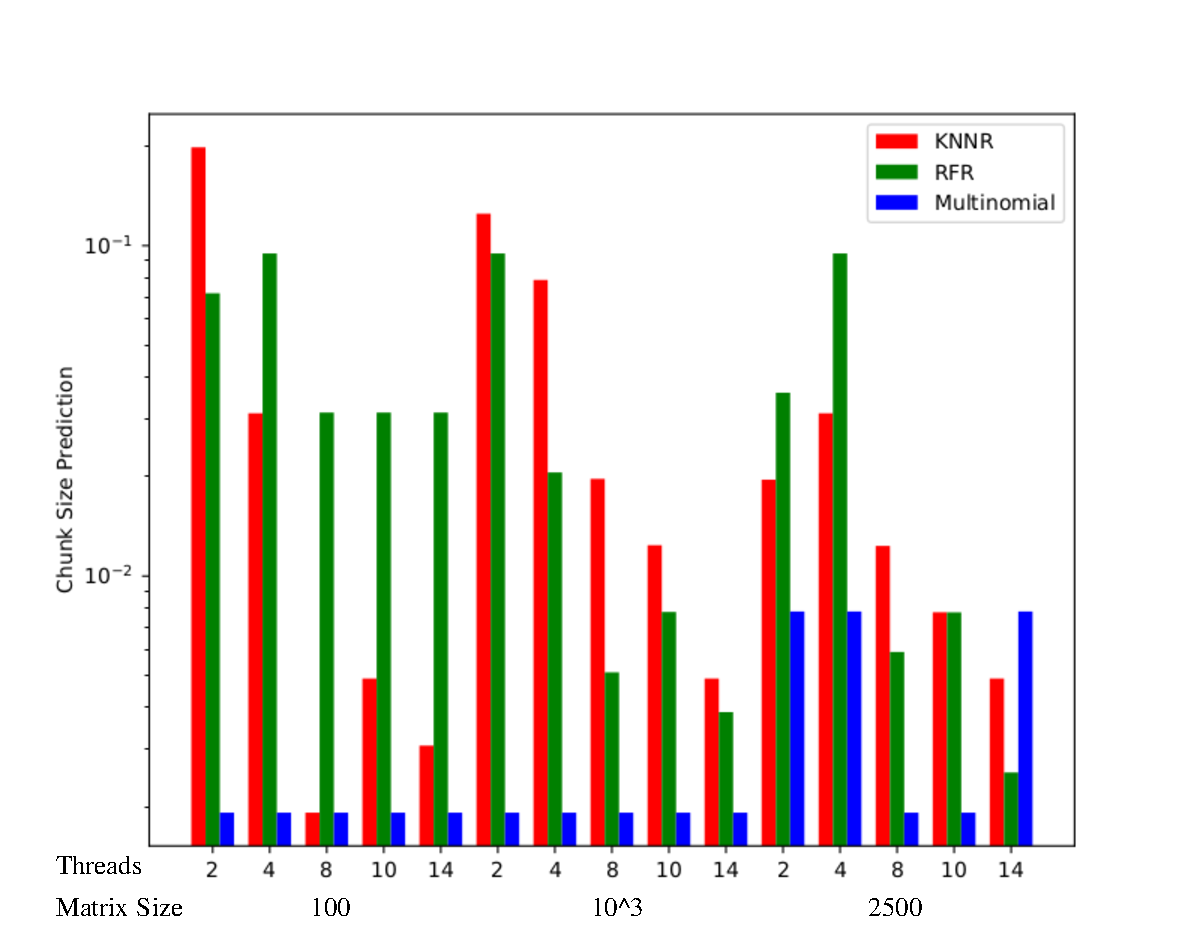
\includegraphics[width=\textwidth]{images/bars_matrix_cs.pdf}
		\caption[Network2]%
		{{Chunk sizes}}    
	\end{subfigure}
	\hfill
	\begin{subfigure}[b]{0.49\textwidth}  
		\centering 
		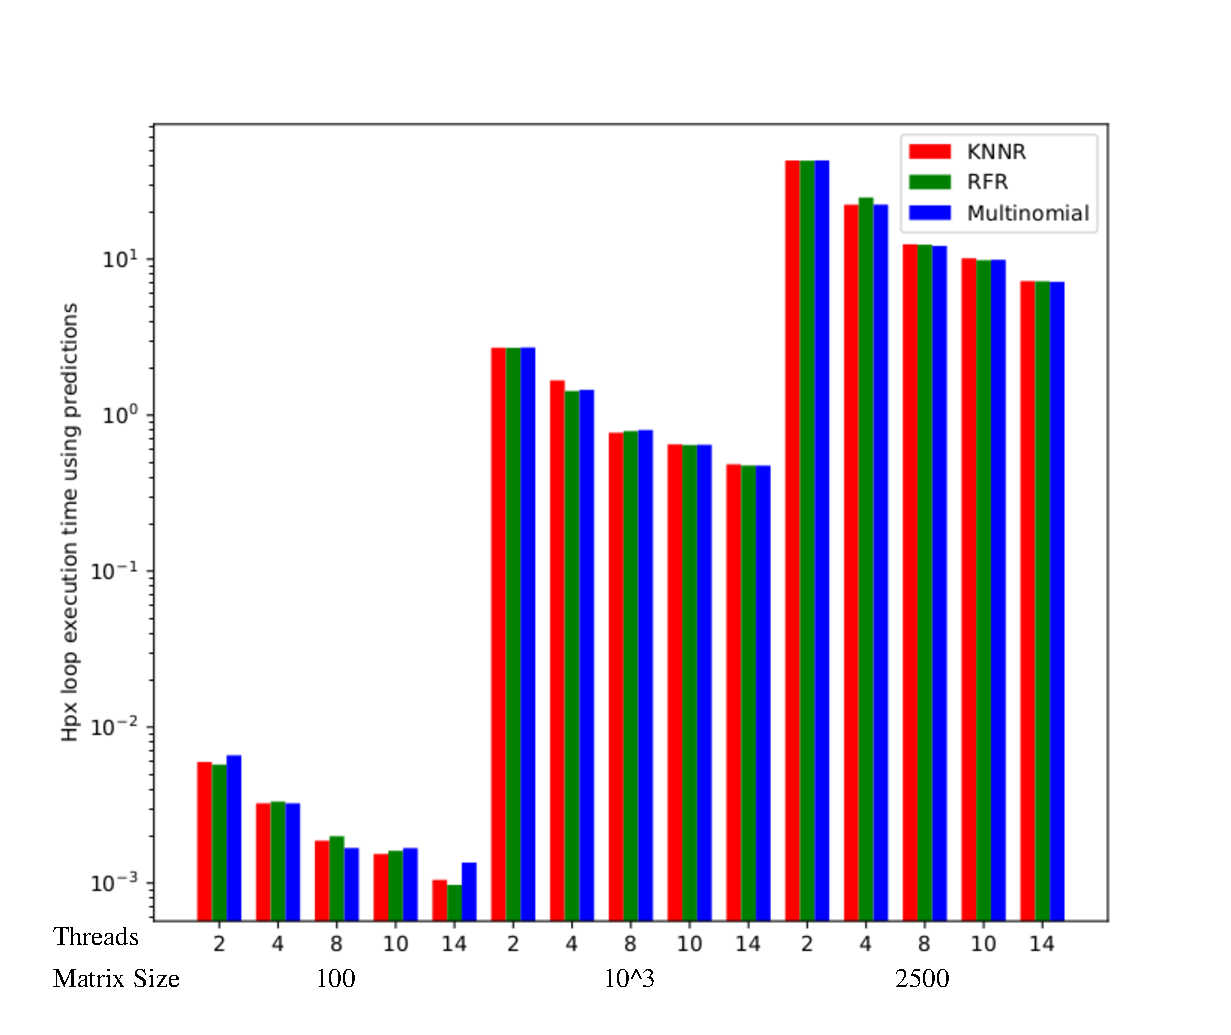
\includegraphics[width=\textwidth]{images/bars_matrix_times.pdf}
		\caption[]%
		{{HPX loops execution times}}    
	\end{subfigure}
	\caption{Chunk sizes predicted by 3 machine-learning algorithms on Matrix-Matrix multiplication functions (a) and the resulting Execution times measured on hpx for-loops (b)} 
\end{figure*}

Table 15 and Figure 21 show that for this function, multinomial algorithm is better than the other two. 
\newpage
\subsubsection{Max}
\begin{table}[h]
	\centering
	\caption{Total execution times (s) on hpx for-loops with the predictions of 3 machine learning algorithms on Max using k-fold cross validation 10 times and comparing with minimal time obtained by taking the minimum time for each experiment on the data-set}
	\label{my-label}
	\begin{tabular}{|c|c|c|c|c|}
		\hline
		& Minimal Time&K-Nearest-Neighbors & Random Forest &Multinomial Class Corrected bias\\ \hline
		k=10  &48.432&
		79.47$\pm$1.33       & 75.52$\pm$1.53&75.7$\pm$1.72 \\ \hline
	\end{tabular}
\end{table}

\begin{figure*}[h]
	\centering
	\begin{subfigure}[b]{0.5\textwidth}
		\centering
		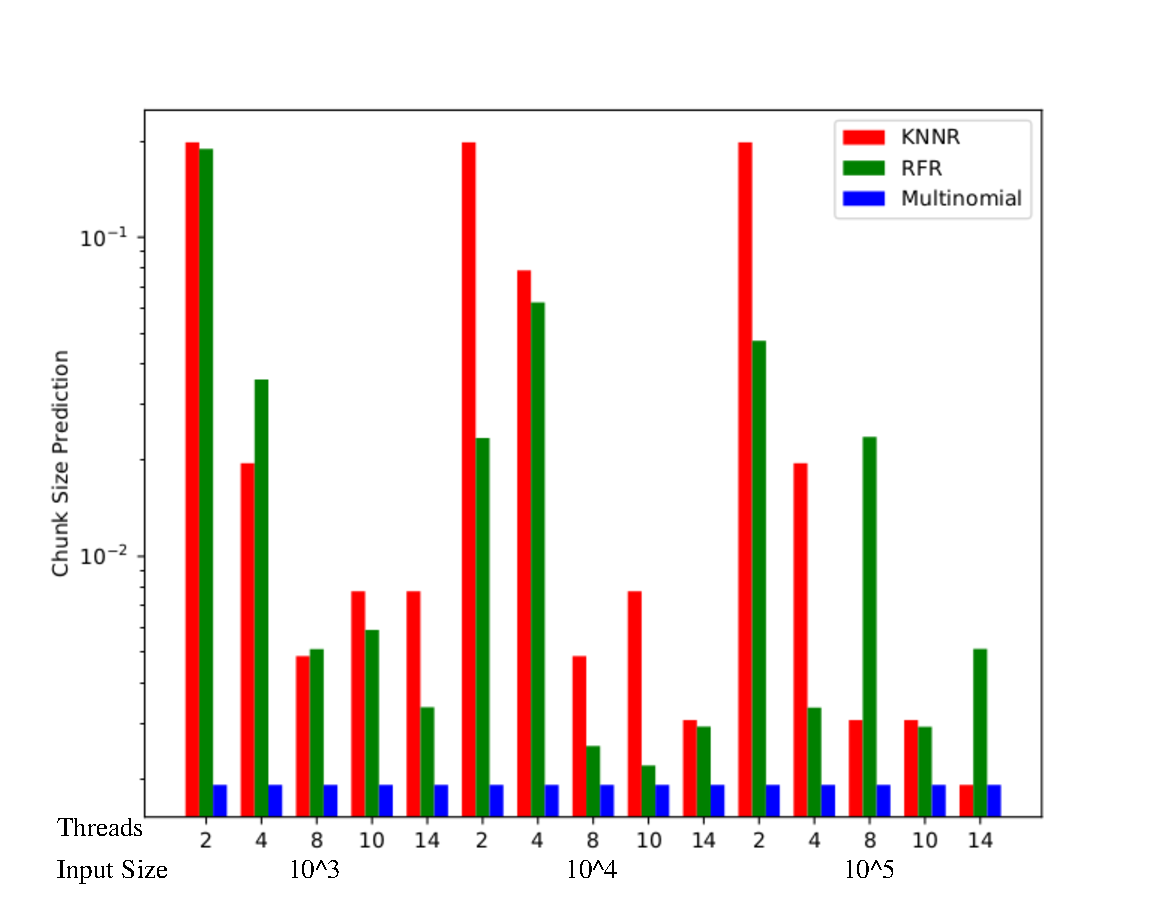
\includegraphics[width=\textwidth]{images/bars_max_cs.pdf}
		\caption[Network2]%
		{{Chunk sizes}}    
	\end{subfigure}
	\hfill
	\begin{subfigure}[b]{0.49\textwidth}  
		\centering 
		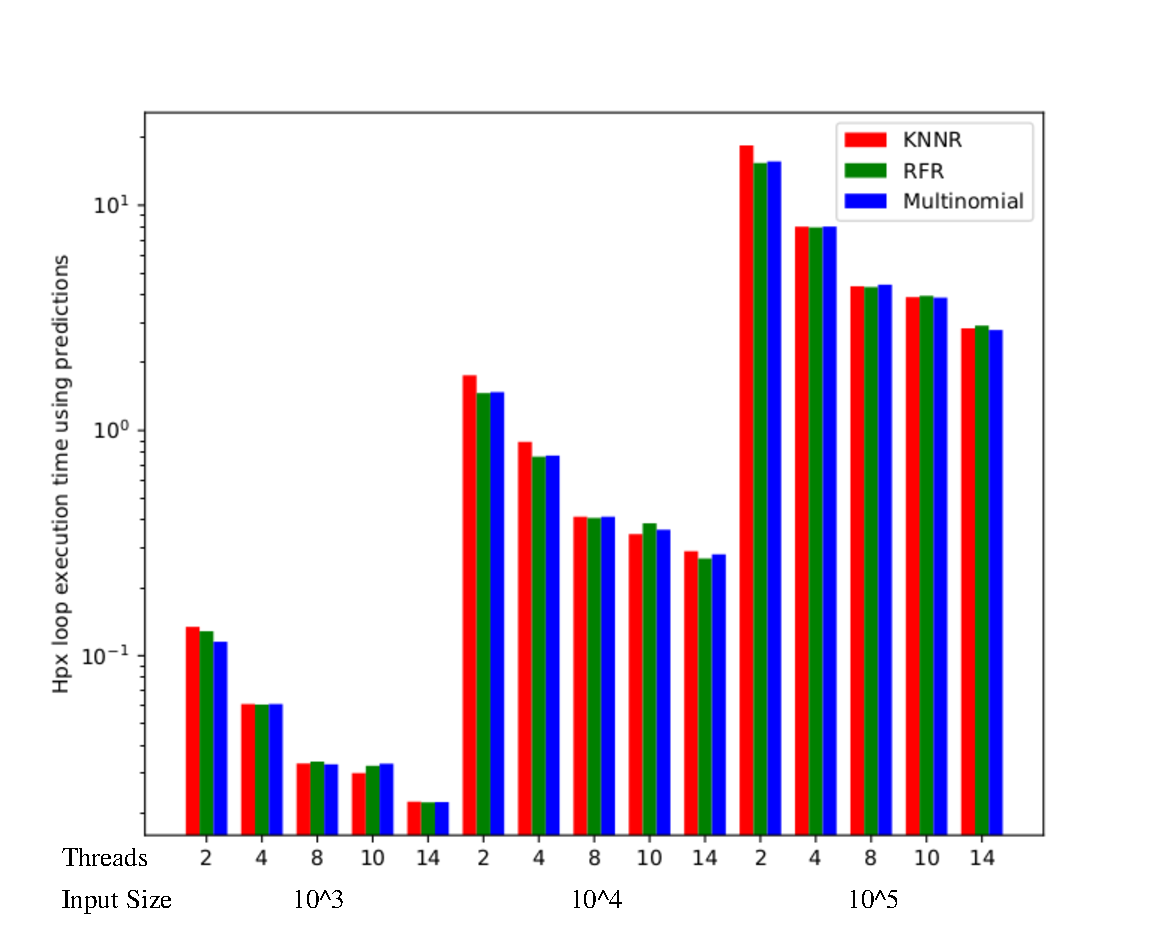
\includegraphics[width=\textwidth]{images/bars_max_times.pdf}
		\caption[]%
		{{HPX loops execution times}}    
	\end{subfigure}
	\caption{Chunk sizes predicted by 3 machine-learning algorithms on Max functions (a) and the resulting Execution times measured on hpx for-loops (b)} 
\end{figure*}
Table 16 and Figure 22 show that multinomial only predicts small chunk sizes while other algorithms are more nuanced. This doesn't seem to affect execution time that much .
\newpage
\subsubsection{Tensor Generator}
\begin{table}[h]
	\centering
	\caption{Total execution times (s) on hpx for-loops with the predictions of 3 machine learning algorithms on Tensor generator function using k-fold cross validation 10 times and comparing with minimal time obtained by taking the minimum time for each experiment on the data-set}
	\label{my-label}
	\begin{tabular}{|c|c|c|c|c|}
		\hline
		& Minimal Time&K-Nearest-Neighbors & Random Forest &Multinomial Class Corrected bias\\ \hline
		k=10  &26.51&
		27.32$\pm$1.328      & 26.95$\pm$1.73&26.91$\pm$1.34 \\ \hline
	\end{tabular}
\end{table}

\begin{figure*}[h]
	\centering
	\begin{subfigure}[b]{0.5\textwidth}
		\centering
		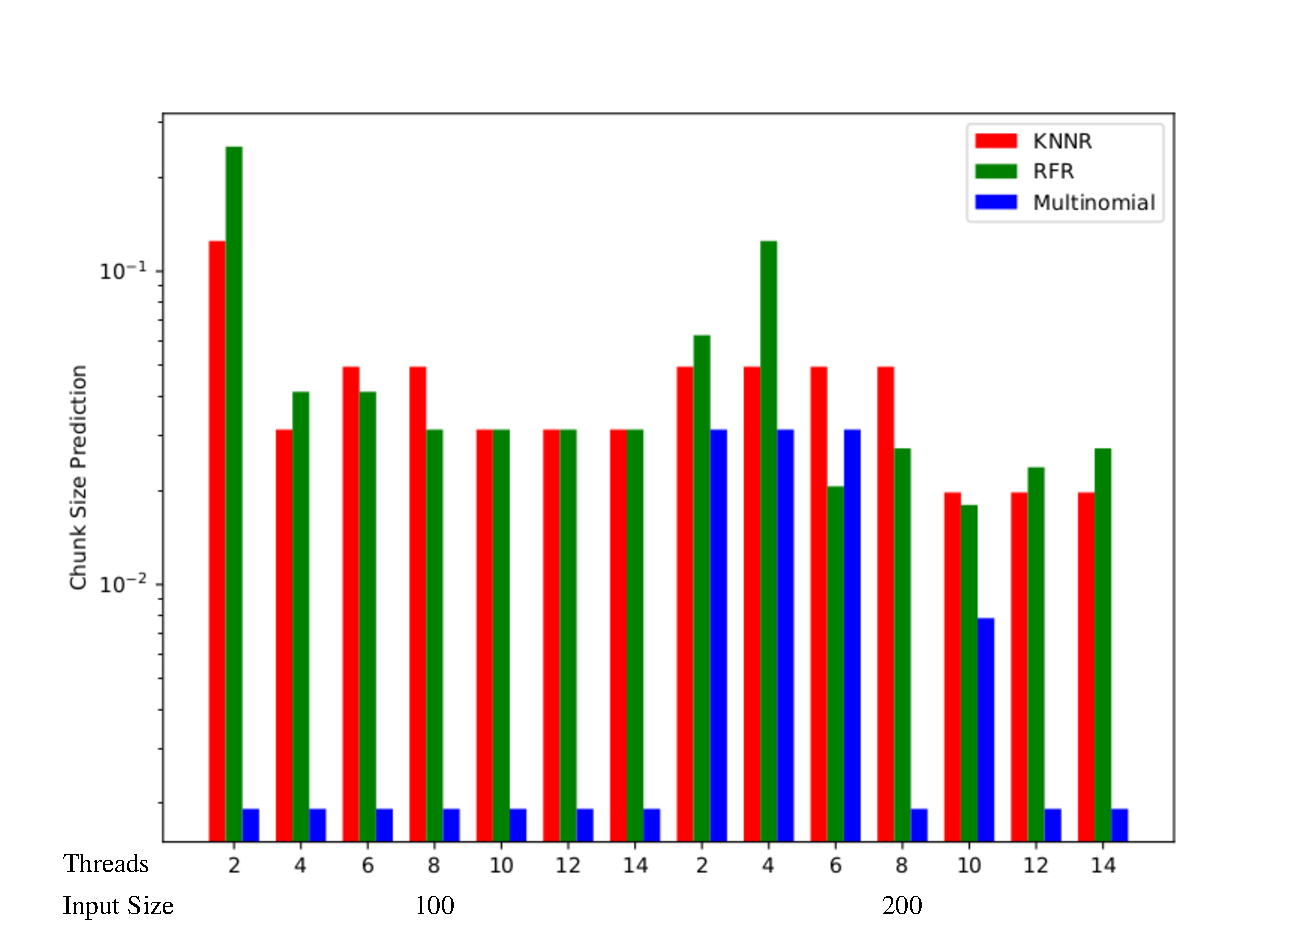
\includegraphics[width=\textwidth]{images/bars_tensor_cs.pdf}
		\caption[Network2]%
		{{Chunk sizes}}    
	\end{subfigure}
	\hfill
	\begin{subfigure}[b]{0.49\textwidth}  
		\centering 
		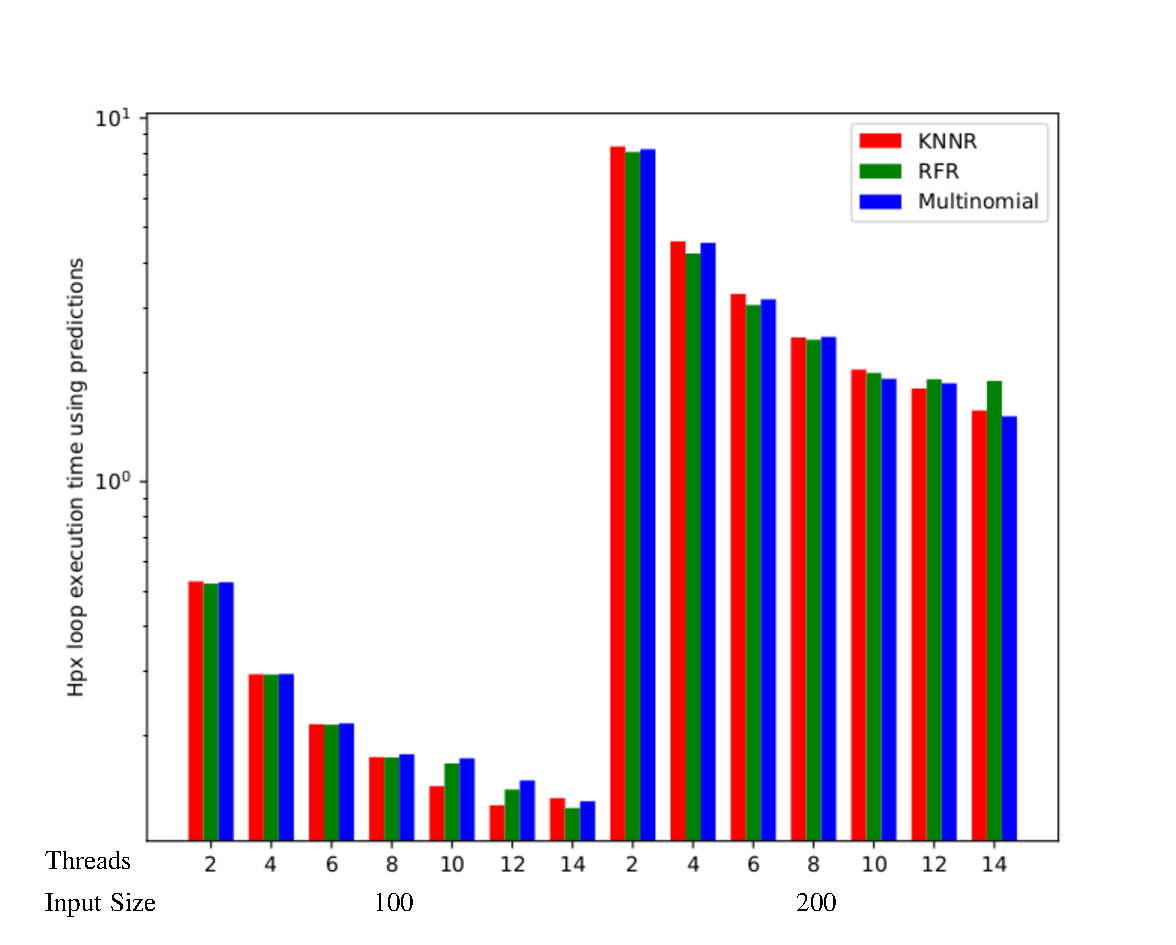
\includegraphics[width=\textwidth]{images/bars_tensor_times.pdf}
		\caption[]%
		{{HPX loops execution times}}    
	\end{subfigure}
	\caption{Chunk sizes predicted by 3 machine-learning algorithms on Tensor Generator functions (a) and the resulting Execution times measured on hpx for-loops (b)} 
\end{figure*}
Table 17 and Figure 23 show that Random Forest and Multinomial, despite differences in predictions,both have the same time.
\section{Conclusion}
The objective of this research was to analyse the relation between loop features and optimal chunk size, and also try to improve the predictions of the Multinomial Classification by usig a regresion algorithm. The hypothesis was that using a regression would reduce the execution time of hpx for-loops since it allows to interpolate between chunk size candidates. However, it was seen that using regression is not significantly better. In fact making improvements to the Multinomial Classification has proven to be as succesfull as using other algorithms. One can wonder why didn't the regression do better. That is simply because for all experiments, close chunk sizes have very close execution times and therefore there is no significant difference between interpolating between candidates or simply choosing candidates from a finite set. According to this research I would say that the next work should focus on the Multinomial Logistic Regression (classification) algorithm. It would still be interesting to keep studying regressions as one would expect them to perform better for very big algorithms where the execution times vary much more with respect to chunk size.

\nocite{*}
\bibliographystyle{ieeetr}
\bibliography{bibliography}





\end{document}